%%%%%%%%%%%%%%%%%%%%%%%%%%%%%%%%%%%%%%%%%%%%%%%%%%%%%%%%%%%%%%%
%% OXFORD THESIS TEMPLATE

% Use this template to produce a standard thesis that meets the Oxford University requirements for DPhil submission
%
% Originally by Keith A. Gillow (gillow@maths.ox.ac.uk), 1997
% Modified by Sam Evans (sam@samuelevansresearch.org), 2007
% Modified by John McManigle (john@oxfordechoes.com), 2015
% Modified by Ulrik Lyngs (ulrik.lyngs@cs.ox.ac.uk), 2018, for use with R Markdown
%
% Ulrik Lyngs, 25 Nov 2018: Following John McManigle, broad permissions are granted to use, modify, and distribute this software
% as specified in the MIT License included in this distribution's LICENSE file.
%
% John tried to comment this file extensively, so read through it to see how to use the various options.  Remember
% that in LaTeX, any line starting with a % is NOT executed.  Several places below, you have a choice of which line to use
% out of multiple options (eg draft vs final, for PDF vs for binding, etc.)  When you pick one, add a % to the beginning of
% the lines you don't want.


%%%%% CHOOSE PAGE LAYOUT
% The most common choices should be below.  You can also do other things, like replacing "a4paper" with "letterpaper", etc.

% This one will format for two-sided binding (ie left and right pages have mirror margins; blank pages inserted where needed):
%\documentclass[a4paper,twoside]{templates/ociamthesis}
% This one will format for one-sided binding (ie left margin > right margin; no extra blank pages):
%\documentclass[a4paper]{ociamthesis}
% This one will format for PDF output (ie equal margins, no extra blank pages):
%\documentclass[a4paper,nobind]{templates/ociamthesis}
%UL 2 Dec 2018: pass this in from YAML
\documentclass[a4paper, nobind]{templates/ociamthesis}


% UL 30 Nov 2018 pandoc puts lists in 'tightlist' command when no space between bullet points in Rmd file
\providecommand{\tightlist}{%
  \setlength{\itemsep}{0pt}\setlength{\parskip}{0pt}}
 
% UL 1 Dec 2018, fix to include code in shaded environments

%UL 2 Dec 2018 reduce whitespace around verbatim environments
\usepackage{etoolbox}
\makeatletter
\preto{\@verbatim}{\topsep=0pt \partopsep=0pt }
\makeatother

%UL 26 Mar 2019, enable strikethrough
\usepackage[normalem]{ulem}

%UL 15 Oct 2019, enable link highlighting to be turned off from YAML
\usepackage[colorlinks=false,pdfpagelabels,hidelinks=true]{hyperref}
%%%%%%%%%%%%%%%%%%%%%%%%%%%%%%%%%%%%%%

\usepackage{titlesec}
\usepackage{tikz}


%%%%% SELECT YOUR DRAFT OPTIONS
% Three options going on here; use in any combination.  But remember to turn the first two off before
% generating a PDF to send to the printer!

% This adds a "DRAFT" footer to every normal page.  (The first page of each chapter is not a "normal" page.)

% This highlights (in blue) corrections marked with (for words) \mccorrect{blah} or (for whole
% paragraphs) \begin{mccorrection} . . . \end{mccorrection}.  This can be useful for sending a PDF of
% your corrected thesis to your examiners for review.  Turn it off, and the blue disappears.
\correctionstrue

%%%%% BIBLIOGRAPHY SETUP
% Note that your bibliography will require some tweaking depending on your department, preferred format, etc.
% The options included below are just very basic "sciencey" and "humanitiesey" options to get started.
% If you've not used LaTeX before, I recommend reading a little about biblatex/biber and getting started with it.
% If you're already a LaTeX pro and are used to natbib or something, modify as necessary.
% Either way, you'll have to choose and configure an appropriate bibliography format...

% The science-type option: numerical in-text citation with references in order of appearance.
% \usepackage[style=numeric-comp, sorting=none, backend=biber, doi=false, isbn=false]{biblatex}
% \newcommand*{\bibtitle}{References}

% The humanities-type option: author-year in-text citation with an alphabetical works cited.
% \usepackage[style=authoryear, sorting=nyt, backend=biber, maxcitenames=2, useprefix, doi=false, isbn=false]{biblatex}
% \newcommand*{\bibtitle}{Works Cited}

%UL 3 Dec 2018: set this from YAML in index.Rmd
\usepackage[style=authoryear, sorting=nyt, backend=biber, maxcitenames=2, useprefix, doi=false, isbn=false, uniquename=false]{biblatex}
\newcommand*{\bibtitle}{Works Cited}

% This makes the bibliography left-aligned (not 'justified') and slightly smaller font.
\renewcommand*{\bibfont}{\raggedright\small}

% Change this to the name of your .bib file (usually exported from a citation manager like Zotero or EndNote).
\addbibresource{references.bib}


% Uncomment this if you want equation numbers per section (2.3.12), instead of per chapter (2.18):
%\numberwithin{equation}{subsection}


%%%%% THESIS / TITLE PAGE INFORMATION
% Everybody needs to complete the following:
\title{\texttt{Red\ de\ economía\ política} ~\\}
\author{INFORME}
\college{La verdad de la gestión del gobierno de Añez}

% Master's candidates who require the alternate title page (with candidate number and word count)
% must also un-comment and complete the following three lines:
%\masterssubmissiontrue
%\candidateno{933516}
%\wordcount{28,815}

% Uncomment the following line if your degree also includes exams (eg most masters):
%\renewcommand{\submittedtext}{Submitted in partial completion of the}
% Your full degree name.  (But remember that DPhils aren't "in" anything.  They're just DPhils.)
\degree{}
% Term and year of submission, or date if your board requires (eg most masters)
\degreedate{Bolivia, 7 de agosto 2020}


%%%%% YOUR OWN PERSONAL MACROS
% This is a good place to dump your own LaTeX macros as they come up.

% To make text superscripts shortcuts
	\renewcommand{\th}{\textsuperscript{th}} % ex: I won 4\th place
	\newcommand{\nd}{\textsuperscript{nd}}
	\renewcommand{\st}{\textsuperscript{st}}
	\newcommand{\rd}{\textsuperscript{rd}}

%%%%% THE ACTUAL DOCUMENT STARTS HERE
\begin{document}
\titleformat{\chapter}[display]
  {\normalfont\huge\bfseries\raggedleft}
  {{\fontsize{100}{130}\color{gray}\selectfont\thechapter\rlap{}}}
  {20pt}
  {\Huge}
%%%%% CHOOSE YOUR LINE SPACING HERE
% This is the official option.  Use it for your submission copy and library copy:
\setlength{\textbaselineskip}{22pt plus2pt}
% This is closer spacing (about 1.5-spaced) that you might prefer for your personal copies:
%\setlength{\textbaselineskip}{18pt plus2pt minus1pt}

% You can set the spacing here for the roman-numbered pages (acknowledgements, table of contents, etc.)
\setlength{\frontmatterbaselineskip}{17pt plus1pt minus1pt}

% UL: You can set the line and paragraph spacing here for the separate abstract page to be handed in to Examination schools
\setlength{\abstractseparatelineskip}{13pt plus1pt minus1pt}
\setlength{\abstractseparateparskip}{0pt plus 1pt}

% UL: You can set the general paragraph spacing here - I've set it to 2pt (was 0) so
% it's less claustrophobic
\setlength{\parskip}{2pt plus 1pt}


% Leave this line alone; it gets things started for the real document.
\setlength{\baselineskip}{\textbaselineskip}


%%%%% CHOOSE YOUR SECTION NUMBERING DEPTH HERE
% You have two choices.  First, how far down are sections numbered?  (Below that, they're named but
% don't get numbers.)  Second, what level of section appears in the table of contents?  These don't have
% to match: you can have numbered sections that don't show up in the ToC, or unnumbered sections that
% do.  Throughout, 0 = chapter; 1 = section; 2 = subsection; 3 = subsubsection, 4 = paragraph...

% The level that gets a number:
\setcounter{secnumdepth}{0}
% The level that shows up in the ToC:
\setcounter{tocdepth}{0}
%{1}


%%%%% ABSTRACT SEPARATE
% This is used to create the separate, one-page abstract that you are required to hand into the Exam
% Schools.  You can comment it out to generate a PDF for printing or whatnot.
%\begin{abstractseparate}
%  jose
%\end{abstractseparate}

% JEM: Pages are roman numbered from here, though page numbers are invisible until ToC.  This is in
% keeping with most typesetting conventions.
\begin{romanpages}

% Title page is created here
\maketitle

%%%%% DEDICATION -- If you'd like one, un-comment the following.
%%\begin{dedication}
%  For Yihui Xie
%\end{dedication}
%
%%%%% ACKNOWLEDGEMENTS -- Nothing to do here except comment out if you don't want it.
%%\begin{acknowledgements}
% 	jose
%\end{acknowledgements}
%

%%%%% ABSTRACT -- Nothing to do here except comment out if you don't want it.
%\begin{abstract}
%	jose
%\end{abstract}

%%%%% MINI TABLES
% This lays the groundwork for per-chapter, mini tables of contents.  Comment the following line
% (and remove \minitoc from the chapter files) if you don't want this.  Un-comment either of the
% next two lines if you want a per-chapter list of figures or tables.
%%%
% This aligns the bottom of the text of each page.  It generally makes things look better.
\flushbottom

% This is where the whole-document ToC appears:
\tableofcontents


% Uncomment to generate a list of tables:
%%%%% LIST OF ABBREVIATIONS
% This example includes a list of abbreviations.  Look at text/abbreviations.tex to see how that file is
% formatted.  The template can handle any kind of list though, so this might be a good place for a
% glossary, etc.
\include{front-and-back-matter/abbreviations}

% The Roman pages, like the Roman Empire, must come to its inevitable close.
\end{romanpages}

%%%%% CHAPTERS
% Add or remove any chapters you'd like here, by file name (excluding '.tex'):
\flushbottom

% all your chapters and appendices will appear here

\hypertarget{presentaciuxf3n}{%
\chapter{Presentación}\label{presentaciuxf3n}}

Han transcurrido 9 meses (días menos) desde el 10 y 12 de noviembre 2019 cuando se produjo un golpe de Estado en Bolivia y Janine Añez se autonombró presidenta. Golpe organizado y auspiciado por EE.UU, la oligarquía cruceña y la ultraderecha del país y , acompañados por las fuerzas más reaccionarias de nuestro Continente.

Bolivia vivía hasta esa fecha, uno de sus momentos políticos, económicos, sociales, culturales, más prósperos y de transformaciones estatales estructurales, en razón de los intereses de las grandes mayorías siempre excluidas. Los pueblos originarios campesinos indígenas no solo fueron beneficiarios de políticas de inclusión, redistribución de la riqueza, reducción de la pobreza, acceso a derechos civiles y políticos y también a los derechos económicos, sociales y culturales como nunca en la historia, sino que, fueron protagonistas de esos hechos, fueron el sujeto social de esos cambios.

La lucha de clases durante los casi 14 años siempre estuvo presente, pese a la línea equivocada de invisibilizarla y buscar acercamientos con los intereses del capital, pensando seguramente, que era posible conciliar intereses a bien de seguir avanzando en las transformaciones del proceso de cambio. Mas la vida y la historia es implacable y nos mostró a nosotros, a los bolivianos y a las fuerzas progresistas y de avanzada en América Latina, que los representantes del capital y sus testaferros, no ceden, no concilian, no dejan el campo de la lucha de clases, así sea explicita o camuflada, siempre buscan la derrota de las fuerzas populares y de su proyecto político.

Esto es lo que ocurrió el 10 de noviembre, que fue en realidad, la etapa final de una conspiración desatada desde el mismo día que Evo Morales ganó las elecciones en 2005.

La extrema derecha en Bolivia se hizo del poder a través de un golpe de estado y toda la ilegalidad justificada con la masacre de Senkata, Sacaba y Betanzos. Pero fueron la oligarquía y los empresarios privados agroindustriales, los que realmente manejaron el país en estos meses de pésima gestión gubernamental de facto de Añez y su Gabinete.

¿Qué es realmente los que hicieron durante estos 9 meses?. Añez presentó un informe público donde la obsesión por Evo Morales y la acusación facilona de echar la culpa de todo al MAS no sale de su discurso. Muchos/as con decencia y honestidad intelectual afirmaran con acierto las limitaciones pronunciadas de Añez y la condición estólida de muchos de sus ministros. Sin embargo, existen intereses y personajes no visibles que digitaron las políticas y medidas. Y es precisamente, esas acciones y políticas las que debemos evaluar, por encima de los sujetos desechables que la lógica imperial introduce.

En esa línea, compartimos una revisión crítica y fundamentada de lo que el gobierno de facto realizó en verdad en estos casi nueve meses. Visto en su conjunto, puede darnos la comprensión de cuerpo entero de los intereses neoliberales que se intenta restaurar.

No abordamos muchas problemáticas, en tanto la presente sistematización, es una revisión rápida de la acción gubernamental de la derecha y, por que el pueblo boliviano, conoce, está en su retina, en su memoria y en su piel, la agresividad fascista, racista y retrógrada del gobierno que representa los intereses del capital.

\hypertarget{pacificaciuxf3n-se-violaron-los-derechos-humanos}{%
\chapter{¿Pacificación? ¡Se violaron los derechos humanos!}\label{pacificaciuxf3n-se-violaron-los-derechos-humanos}}

A lectura de la Constitución, un Gobierno Transitorio tiene la única responsabilidad de convocar en el tiempo prudente, a nuevas elecciones y esa era según norma, la función de Añez. Pero respaldada por su gabinete, la Policía y FF.AA. golpistas, al viejo estilo de las dictaduras militares desató una represión sañuda contra el pueblo movilizado desde las vísperas del 10 de noviembre.

El golpe de Estado de noviembre 2019 instauró un régimen a la cabeza de Jeanine Añez cuya sistemática violación de derechos humanos es la característica esencial del gobierno transitorio. La pacificación del país y el llamado a elecciones fueron las únicas tareas que debía realizar en el plazo inmediato.

A casi 9 meses del gobierno de facto ni la pacificación ni el llamado a elecciones se han cumplido, con un gobierno transitorio que utiliza la pandemia para prorrogarse en el poder. Vivimos como lo ha calificado el profesor Raúl Zaffaroni en un Estado de No Derecho y que ha llevado al país a una crisis política, social, económica y de derechos humanos sin precedentes.

El régimen ostenta el triste récord de ser uno de los gobiernos más denunciados por vulneración de derechos humanos en el mundo, en tan sólo 9 meses de gestión. Desde órganos como la Comisión Interamericana de Derechos Humanos (CIDH), la Relatoría para la Libertad de Expresión, el Alto Comisionado para los Derechos Humanos de NNUU, el Relator Especial de la ONU sobre la Independencia de Magistrados y Abogados, el Experto Independiente sobre las consecuencias de la deuda externa de la ONU, hasta organismos de reconocida trayectoria como Amnistía Internacional o Human Rights Watch, sólo por nombrar algunos, todos se manifestaron condenando las violaciones de derechos humanos en Bolivia, generando una imagen a nivel internacional de un régimen contrario a los derechos humanos. Recopilamos algunas de las mayores violaciones en este campo:

\begin{enumerate}
\def\labelenumi{\arabic{enumi}.}
\item
  \textbf{Masacre de Sacaba, Senkata, Vetanzos y otros asesinatos en la zona sur}. Constituyen los hechos más graves de vulneración de derechos humanos, con más de 30 muertos, 800 heridos y cientos de detenidos. Son calificados como masacres por la Comisión Interamericana de Derechos Humanos (CIDH), lo cual implica que son Crímenes de Lesa Humanidad, susceptibles de ser perseguidos internacionalmente, por ejemplo ante la Corte Penal Internacional. Estos hechos se dieron al poco tiempo de la autoproclamación de la Sra. Áñez y fueron precedidos por el DS 4078 de 14 de noviembre de 2019, un día antes de la masacre de Sacaba, que exime de responsabilidad penal a las fuerzas militares y policiales. En las masacres se verificaron además torturas y desapariciones forzosas. A julio de 2020, las investigaciones no han avanzado y se cierne un manto de impunidad en estos gravísimos hechos. Los asesinatos de la zona sur en Ovejuyo, Pedregal, Rosales y Chasquipampa, se dan poco antes del 12 de noviembre y hasta ahora han quedado sin ninguna investigación.
\item
  \textbf{Persecuciones políticas}. La persecución judicial y política es una de las expresiones más evidentes de este gobierno de facto como parte de su estrategia de guerra jurídica (lawfare), es decir, la utilización de la justicia con fines políticos. La persecución judicial y política se inició contra partidarios del MAS, dirigentes sociales y cualquiera que osara desafiar al gobierno de facto. Los delitos frecuentes por el que se iniciaron las persecuciones fueron sedición, terrorismo, corrupción, características típicas del lawfare. Destacamos la persecución política contra Patricia Hermosa, ex Jefe de Gabinete de Evo Morales; a los siete asilados en la Residencia de México a quienes les niegan lo salvoconductos, a pesar de que México ya concedió el asilo; al candidato de MAS-IPSP, Luis Arce, con el fin de inhabilitarlo; al propio ex Presidente Evo Morales, con el mismo fin; a Facundo Molares, periodista argentino acusado de pertenecer a las FARC y haber organizado las movilizaciones de octubre y noviembre, sin pruebas!!.
\item
  \textbf{Exacerbación del odio y del racismo}. El odio y el racismo son las características del régimen, si bien se intentó disimular, viene precedido por la quema y ofensa a la wiphala, la suspensión y ataque a las 53 radios comunitarias. La propia presidenta de facto manifestó ``Debemos impedir que retornen los salvajes''.
\item
  \textbf{No ingreso a compatriotas}. En un hecho sin precedentes, con la excusa de la cuarentena, se impidió el retorno de cientos de bolivianos (entre ellos mujeres embarazadas, adultos mayores y niños) que retornaban de Chile por tierra, se le impidió el paso argumentando que ponían en riesgo la salud de los demás. Ninguno tenía COVID y tuvieron que esperar semanas para ingresar. En contrapartida, días antes se permitió el retorno de bolivianos que llegaban por avión, e incluso se les permitió hacer la cuarentena en sus domicilios. Vulnerando los derechos de los primeros y creando ciudadanos de primera y de segunda.
\item
  \textbf{Libertad de expresión}. Mediante varios decretos supremos el gobierno con la excusa del Covid-19 restringió la libertad de expresión estableciendo sanción penal a la persona que desinforme sobre la pandemia, incluyendo expresiones artísticas. Esta grave vulneración de la libre expresión fue observada por la Relatoría de Libertad de Expresión y por la organización Human Rights Watch y de cientos de organizaciones en Bolivia. A raíz de estos decretos, varios ciberactivistas también fueron detenidos, acusados de atentar contra la salud. La presión social obligo al gobierno transitorio a derogar los decretos.
\item
  \textbf{Derecho la salud}. La pandemia fue utilizada por el gobierno para la vulneración de derechos humanos y para prorrogarse en el poder. A pesar de señalar que su lucha es por la salud contra el Covid 19, su incapacidad ha llevado a una catástrofe sanitaria en el país, sin respiradores, sin medicamentos, sin pruebas masivas, sin laboratorios, lo cual se constituye en un atentado directo a la salud. Bolivia está entre los diez países del mundo que peor gestiona la pandemia (New York Times).
\item
  \textbf{Derecho a la educación}. Al igual que la salud es la primera función del Estado, que tiene la obligación de sostenerla, gestionarla y garantizarla. La incapacidad e irresponsabilidad del gobierno transitorio la llevó a una de sus peores crisis en los últimos años, sin lograr acuerdos con los maestros ni con los padres de familia sobre todo para acceder a una educación virtual que alcance a todos. Finalmente, sin poder hallar soluciones terminan clausurando el año escolar, dañando a millones de estudiantes que se quedan privados de este derecho, en incertidumbre por el futuro de sus estudios. No existe gobierno en el mundo donde la emergencia de la pandemia haya llevado a quitar la educación de su niñez y juventud como el de Añez.
  Se reducido en 35\% la matriculación de estudiantes universitarios en las U. privadas de todo el país por carencias tanto de ingresos para pagar la matriculación y pensiones mensuales, como para muñirse de los equipos tecnológicos suficientes para pasar clases virtuales (Fuente: Diario Pagina Siete). Estas últimas limitaciones están sufriendo con mayor razón, los universitarios de las U. estatales, cuya gran mayoría proviene de sectores con relativamente menores ingresos familiares y/o personales.
\item
  \textbf{Derechos políticos}. Uno de los derechos más afectados por el gobierno transitorio, fue el derecho a tener elecciones de manera oportuna. El gobierno con la excusa de la cuarentena intentó que se postergarán indefinidamente éstas (se postergaron en más de 3 oportunidades), privando de un derecho político fundamental: contar con un gobierno legítimo y democráticamente elegido. Decenas de países celebraron elecciones durante la cuarentena; el más reciente ejemplo, el de República Dominicana el 5 de julio pasado que no significó el aumento de contagios. Por otro lado, impiden las elecciones pero obligan a que cientos de bolivianos hagan filas en bancos, mercados, servicios o para acceder a garrafas de gas, cuando a todas luces, el día de las elecciones es el día que no existe viajes, comercio, tiendas, mercados, transporte, actividades sociales, colas en los bancos, etc, etc. A esta vulneración de derechos se ha sumado el TSE que de manera ilegal, arbitraria e inconsulta fijó una nueva fecha de elecciones sobrepasando a la Asamblea Legislativa Plurinacional.
\item
  \textbf{Destrucción de las empresas estatales en especial YPFB}. Recursos naturales. Los recursos naturales y su manejo adecuado constituyen la base material de los derechos humanos como lo señalan los principales pactos internacionales de derechos humanos. Por ello, el daño a las empresas estatales por parte del gobierno de facto, en particular de YPFB, la empresa estatal más importante de Bolivia, con casos de corrupción, malos manejos, negociaciones contrarios a los intereses del país, ponen en vilo el futuro del país y la vigencia de los derechos humanos. En esta misma línea, preocupan las gestiones para la entrega del litio a intereses foráneos. Los atentados y desmantelamiento de la estabilidad económica y las empresas estatales dejadas por el proceso de Cambio, están directamente relacionados con los Derechos Económicos, Sociales y culturales (DESC), en tanto los DESC solo pueden materializarse con una redistribución de la riqueza, misma que solo puede ser possible si el país y su economía es soberana, es autónoma de los intereses de las transnacionales y es patriótica.
\item
  \textbf{Estan convocados entonces los intelectuales sensibles}, las organizaciones populares, la dirigencia sindical, las Universidades, la academia, los politicos, las regiones, la juventud y todo el pueblo, a una lectura crítica de una parte de nuestra historia reciente que se encuentra en el Informe Preliminar de la CIDH del 10 de diciembre de 2019, en el Informe Final de la Delegación Argentina en Solidaridad con el Pueblo Boliviano de diciembre de 2019, en el reciente Informe ``Nos dispararon como a animales'' de la Clínica Internacional de Derechos Humanos de Harvard de la Red Universitaria por los Derechos Humanos, que dan cuenta de manera sistematizada de las graves violaciones de derechos humanos del gobierno de facto, conforme al Derecho Internacional de los Derechos Humanos.
\end{enumerate}

\hypertarget{el-desgobierno-y-la-ineptitud-en-la-salud}{%
\chapter{El desgobierno y la ineptitud en la salud}\label{el-desgobierno-y-la-ineptitud-en-la-salud}}

La gestión desastrosa en materia de salud puede resumirse en los siguientes hechos:

\begin{enumerate}
\def\labelenumi{\arabic{enumi}.}
\item
  Liquidación y archivo del Sistema Único de Salud Universal y Gratuito, puesto en vigencia en el país desde el mes de febrero mediante la promulgación de la Ley 1152, que significaba la atención universal y gratuita para más de 7 millones de bolivianos y bolivianas no protegidos por los entes gestores de la seguridad social de corto plazo.
\item
  Falta de transparencia en el uso de los recursos programados destinados a las atenciones del Sistema Único de Salud y al fortalecimiento de la infraestructura y el equipamiento de los hospitales públicos y a la asignación de mayores recursos humanos para la salud. En el cuadro siguiente se registran los recursos destinados al SUS, según gestiones.
\end{enumerate}

\begin{figure}

{\centering 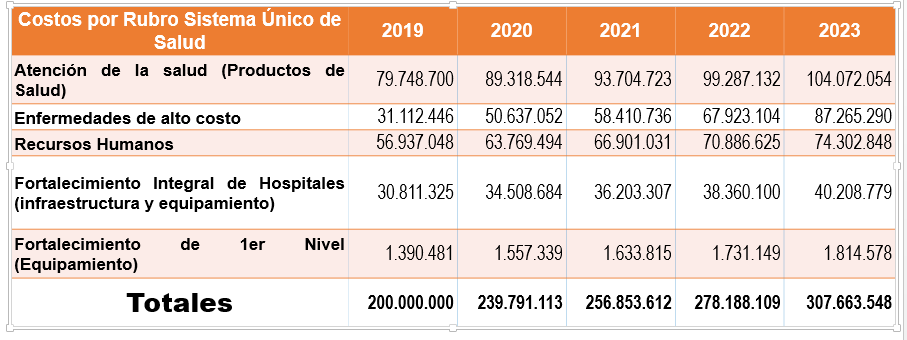
\includegraphics[width=1\linewidth]{figures/tabla-salud} 

}

\caption{Recursos destinados al SUS}\label{fig:unnamed-chunk-1}
\end{figure}

\begin{enumerate}
\def\labelenumi{\arabic{enumi}.}
\setcounter{enumi}{2}
\item
  En la práctica, Jeanine Añez ha estado utilizando estos recursos en la entrega de nuevos ítems y algún equipamiento, cuando estos recursos ya estaban programados en forma creciente hasta la gestión 2023.
\item
  Acoso, persecución, apresamiento y, finalmente, retiro de 700 profesionales de la Brigada Médica Cubana en Bolivia, que se había constituido en un importante paliativo al enorme déficit histórico de salud de Bolivia. Desde 2005, la Brigada Médica Cubana en Bolivia ha realizado 73 millones de consultas y millón y medio de operaciones quirúrgicas (1), ha atendido 60 mil partos y ha salvado 110 mil vidas (2). El retiro de la Brigada en Bolivia ha dejado sin atención gratuita y de alto nivel profesional a los más pobres de nuestro país. La permanencia de la Brigada Médica Cubana en el país, en las actuales circunstancias de la pandemia por el coronavirus, habría sido indudablemente de gran apoyo para contención de la misma.
\item
  El Gobierno de facto de Jeanine Anez liquidó importantes programas nacionales del Ministerio de Salud, como el de Salud Familiar Comunitaria Intercultural-Mi Salud (Programa SAFCI-Mi Salud), Bono Juana Azurduy, Telesalud y otros, procediendo al despido de profesionales de estos programas, especialmente al despido de médicos bolivianos graduados en la Escuela Latinoamericana de Medicina (ELAM) de la República de Cuba. El blanco del cierre fueron sobre todo los programas del primer nivel de atención que estaban dirigidos a la promoción de la salud y a la prevención de la enfermedad.
\item
  Falta de transparencia en el uso de los recursos. Con motivo de la Pandemia por el coronavirus el país recibió donaciones internacionales, además del retiro de fondos del Banco Central de Bolivia. En el mes marzo, Añez anunció que diversos países de la comunidad internacional (Italia, China) comprometieron más de 100 millones de dólares (euros) para la adquisición de material médico para combatir el coronavirus. Sin embargo, el destino y uso de estos recursos no se conocen hasta ahora.
  Como consecuencia de la Pandemia, el Banco Mundial puso a disposición del Gobierno de facto la suma US\$170 millones de disponibilidad inmediata, como parte del préstamo destinado al fortalecimiento de redes de salud. Tampoco se conoce el uso y destino de estos recursos.
\item
  Corrupción. Una característica que resalta a los nueve meses del gobierno de facto es la corrupción. Hasta los obispos de la iglesia católica se han visto obligados a pronunciarse al respecto, expresando que la compra de respiradores artificiales, cuyo costo es \$us. 6.600 la unidad según su fabricante español, fueron adquiridos en \$us.27.000 por el Ministerio de Salud, operación que le costó a Bolivia más de \$us. 5 millones. Además del importante daño económico que este acto de representa para el país, mucho más importante es el daño a la salud del pueblo boliviano, pues hasta ahora la adquisición de esos respiradores para las Unidades de Terapia Intensiva no llegó nunca a los servicios de salud y no se dispone de los respiradores que podrían salvar muchas vidas de los afectados por el coronavirus. El escándalo de corrupción por sobreprecio en la adquisición de 170 respiradores, de conocimiento de todo el país, dio como resultado el encarcelamiento del exministro Navajas principal sindicado de este acto de corrupción y de otros funcionarios del Ministerio de Salud. Mientras tanto, el ex ministro de salud, Marcelo Navajas, bien gracias, en prisión preventiva en una clínica privada.
\item
  Inestabilidad e improvisación en la designación de ministros de salud. Desde el 10 de marzo, fecha en la que se reportan los dos primeros casos de coronavirus en el país se ha tenido 4 ministros de salud: El primero Dr.~Aníbal Cruz, del Colegio Médico de Bolivia, como premio a la participación de los gremios de salud en el Golpe de Estado, quien tuvo que renunciar el 8 de abril, en plena pandemia y cuando en el país ya teníamos 200 casos confirmados y 15 muertos a causa del COVID-19. En la misma fecha, la Sra. Jeanine Añez, posesiona en el cargo de Ministro de Salud al Dr.~Marcelo Navajas Salinas, médico de Embajada Americana y propietario de clínicas privadas. Actualmente, el Dr.~Navajas, ex ministro de salud, se encuentra con detención domiciliaria, acusado por corrupción en la compra de 170 respiradores con sobreprecio. Desde el 20 de mayo, la Dra. Heidy Roca, del Servicio Departamental de Salud de Santa Cruz, asume el cargo de Ministra de Salud en forma interina. Finalmente, el 10 de julio el ministro interino de Defensa de Bolivia, Luis Fernando López, militar de profesión, es nombrado en forma irresponsable como la cabeza del Ministerio de Salud (!!), en tanto dure la recuperación de la ministra interina de esa repartición Heidy Roca, que contrajo la COVID-19. En estas condiciones no se podía esperar que la salud de la población y la pandemia por el coronavirus sean adecuadamente gestionadas.
\item
  Improvisación en la gestión de la pandemia por el coronavirus. Centrado en el modelo biomédico, el gobierno aparentemente se preocupó más en la preparación de los servicios de salud para la atención hospitalaria de los casos del COVID-19. La carencia de pruebas de laboratorio para el diagnóstico de la COVID-19, que es otra de las negligencias de este gobierno, no ha permitido, y no permite hasta ahora, conocer el número real de contagiados por el coronavirus en el país. En estas condiciones, tampoco es posible desarrollar acciones efectivas de contención de la pandemia, por más cuarentenas que se hagan.
\item
  La aparición de casos graves de COVIB-19, como ocurrió en los departamentos de Santa Cruz y Beni, ha puesto en evidencia que el gobierno no ha tomado las precauciones del caso para enfrentar los casos más graves del COVID-19. Los servicios de terapia intensiva existentes y los que el gobierno dice haber implementado han colapsado en estos departamentos.
\item
  El Sistema Único de Salud Universal y Gratuito fue creado para proteger la salud de los bolivianos, inclusive contra epidemias y desastres. Fue preparado fortaleciendo el Sistema con infraestructura, equipos y recursos humanos y debía tener un presupuesto de 1.700 millones de bolivianos para la presente gestión, los mismos que deberían ser empleados para el control y atención de las epidemias de Dengue y COVID-19. Se deberían emplear los recursos del Sistema Único de Salud en la provisión gratuita a la población de barbijos y alcohol en gel. Estos recursos deberían también emplearse para la compra de suficientes pruebas y preparar establecimientos específicos para la atención de los casos graves de COVID-19, con las medidas más estrictas de bioseguridad para el personal de salud que atienda esta epidemia.
\item
  Al actual gobierno y al Ministerio de Salud jamás se les ha ocurrido la participación comunitaria, la participación de las organizaciones barriales y de otras formas de organización popular en la vigilancia y el control epidemiológico de la pandemia. Las potencialidades del modelo de atención de la Política SAFCI han sido intencionalmente ignoradas. El Programa SAFCI-MI SALUD, -una de cuyas actividades principales era realizar la regular y programada visita familiar y el uso de la carpeta familiar- ha sido, en la práctica abandonada y borrada del quehacer del ministerio de salud, cuando en las actuales circunstancias habría sido un instrumento de gran utilidad y mucha efectividad en la contención de la pandemia.
\end{enumerate}

\hypertarget{la-afectaciuxf3n-a-los-derechos-de-las-y-los-trabajadores.}{%
\chapter{La afectación a los derechos de las y los trabajadores.}\label{la-afectaciuxf3n-a-los-derechos-de-las-y-los-trabajadores.}}

El régimen de facto desde el mismo 10 de noviembre de 2019 desató una persecución en contra de la dirigencia sindical, desconocimiento montado de organizaciones, intervenciones de sedes sindicales, golpizas, amenazas, sin descontar dirigentes pagados a fin de debilitar las movilizaciones y la fuerza popular. Políticamente, se operó como en las dictaduras, con la represión; laboralmente, se despidieron a miles de servidores públicos bajo sospecha de ser militantes del MAS, sin consideración a su antigüedad, necesidad de trabajo y experiencia técnica.

De marzo adelante, con la pandemia, el desorden de la gestión sanitaria y la cuarentena para los sanos y no para los enfermos, las empresas, comercio, y todas las actividades productivas del empresariado privado que se sumaron de memoria a las cuarentenas rígidas y flexibles, terminaron asfixiando la actividad productiva y provocando una recesión acelerada en el país. Hoy, pese a las políticas privilegiadas para la empresa privada, solo pensando en sus intereses, están despidiendo a cientos y miles de trabajadores de sus fuentes laborales.

\begin{enumerate}
\def\labelenumi{\arabic{enumi}.}
\tightlist
\item
  La desocupación que a marzo -antes de la cuarentena- llegó a 7.3\%, ha ascendido en la actualidad a cerca de 9.5\% o más, con más de 400 mil desocupados. Para no perder la memoria, hasta el último día del gobierno de Evo Morales, la desocupación en Bolivia que era la más baja de la región, llegó a 4.5\%.
\end{enumerate}

El instrumento estatal de protección de los trabajadores asalariados y no asalariados como es el Ministerio de Trabajo, ¿cómo puede defenderles si el gobierno es de los empresarios?. El proceder en la política social, delata los intereses que se defiende. Revisemos estas normas atentatorias a los derechos laborales:
Resolución Ministerial Nº 220/20 de 24 de abril de 2020, Ministerio de Trabajo, Empleo y Previsión Social, Reglamentación del teletrabajo:

\begin{itemize}
\tightlist
\item
  Obliga a la suscripción de una ``Adenda o Contrato'', disposiciones normativas que están siendo utilizadas por los empleadores en desmedro de los derechos adquiridos de los trabajadores y obligarles a suscribir un nuevo contrato de trabajo para desconocer su antigüedad, vacaciones acumuladas, etc.
\item
  Incorpora una definición de que en la relación laboral se implementará la evaluación de gestión por resultados, esa medida le significa reducir al trabajador como recurso y podría prescindirse de sus servicios si no hay resultados.
\item
  Con anterioridad en el desarrollo de las relaciones laborales, si se incrementaba la producción, daba lugar al pago del bono de producción, pero siempre mediante acuerdo, ahora este bono sería discutible pero el empleador puede incrementar el trabajo,
\item
  Se establece la definición de ``caso fortuito'' y ``fuerza mayor'' que apertura la posibilidad de su aplicación aduciendo hechos nuevos, un informe de contabilidad fabricado con aprobación del directorio de una empresa. Ya se puede justificar un despido e incluso se puede utilizar para la reducción de algunas conquistas sociales.
\item
  Lo descrito, también puede dar lugar a que el empleador aplique la norma para para la compensación de horas en los centros de trabajo donde se hubiesen reducido horas de trabajo por disposición legal.
\end{itemize}

\begin{enumerate}
\def\labelenumi{\arabic{enumi}.}
\setcounter{enumi}{1}
\tightlist
\item
  Resolución Ministerial N° 229/20 de 18 de mayo de 2020, Ministerio de Trabajo, Empleo y Previsión Social.
\end{enumerate}

\begin{itemize}
\item
  En su artículo 4 establece que tanto el sector público y privado deben adoptar medidas administrativas para contener el contagio y propagación del Coronavirus COVID - 19, debiendo otorgar a los trabajadores y/o servidores públicos aspectos mínimos de bioseguridad, estableciendo el teletrabajo y en caso de que este no se pudiera dar el trabajador tendrá que solicitar vacaciones en el caso de que la institución o empresa cuente dentro de su personal a mayores de 65 años de edad, mujeres embarazadas o con patologías de base crónicas.
\item
  Establece obligaciones al teletrabajador imponiéndole el 100\% de la responsabilidad de dicho trabajo y de la información generada por dichas funciones; señala también que el teletrabajador tiene que cumplir con los protocolos de seguridad establecidos, sin embargo no se conocen estos protocolos, si ya están aprobados, en qué consisten y quién o quiénes serás los responsables del manejo de los mismos.
\item
  Con relación a la solicitud de vacaciones para realizar los trabajos o funciones asignadas, no se puede tratar de vulnerar este derecho al cambiar su naturaleza o finalidad, menos aun cuando se le pide realizar las mismas funciones al trabajador y cumplir horarios de trabajo al empleado cuando está haciendo uso de sus vacaciones.
\end{itemize}

\begin{enumerate}
\def\labelenumi{\arabic{enumi}.}
\setcounter{enumi}{2}
\tightlist
\item
  Decreto Supremo Nº 4272 de 23 de junio de 2020.
\end{enumerate}

Esta norma pretende ser un 21060 remozado, debido a que instruye un despido masivo en el Gobierno, el Artículo 83 establece la reducción de Consultores en línea en las instituciones públicas del nivel central del Estado. Así mismo, el artículo 85 respecto a las medidas para optimizar la gestión empresarial, establece que se adoptará medidas necesarias para optimizar la gestión empresarial pública siendo estas: una política de reducción de gasto corriente del sector público y la optimización de recursos; así como un Plan de Restructuración Administrativa.

\begin{enumerate}
\def\labelenumi{\arabic{enumi}.}
\setcounter{enumi}{3}
\tightlist
\item
  Problemática social y económica de los trabajadores
\end{enumerate}

Los últimos 8 meses además se ha identificado las siguientes problemáticas:

\textbf{Desempleo}.
Según datos del INE de la Nación Andina se ha registrado un aumento adicional de desempleo del 4,83 \% durante el último trimestre de 2019, esto relacionado a que el gobierno de facto de Añez no ha podido mantener el funcionamiento de entidades Estatales, contribuyendo a que la cifra ascienda.
\textbf{Despidos masivos en relación a la pandemia}.
Esto en virtud a la medida radical de cuarentena rígida asumida por Añez, misma que fue realizada sin hacer una evaluación del impacto económico en el País.

\textbf{Inestabilidad política- alto índice de corrupción}.
Generada por el golpe de Estado, alto índice de corrupción y constantes cambios de autoridades Ejecutivas entorno al gobierno de facto.

\textbf{Endeudamiento público}.
El Gobierno De facto de AÑEZ ha procedido a endeudar al País sin tener medidas de reactivación económica, aspecto que a la larga generará despidos masivos.

\textbf{Daño económico a empresas públicas estratégicas}.
Los actos de corrupción del Gobierno de facto han dañado gravemente la Economía de las Empresas Públicas y Estratégicas, claro ejemplo de esto: BOA y ENTEL , aspecto que ha generado desempleo masivos e inestabilidad laboral.

\textbf{Casos emblemáticos}:

\begin{itemize}
\item
  Cerca de 200 trabajadores de la fábrica textilera Altifibers, enclavada en la región de El Alto, se presentaron a trabajar, enterándose en el acto que habían sido despedidos. Los operarios de dicha fábrica han protestado reiteradamente, ya que se les deben sus jornales correspondientes a marzo y abril y ahora se les despide, sin que el gobierno de facto haya emitido pronunciamiento al respecto. El dirigente de los trabajadores de la terxtilera Altifibers, Ángel Mamani, denunció que todos los trabajadores fueron despedidos en medio de la cuarentena por el coronavirus, cuyol gerente general ha hecho conocer un memorándum aduciendo que la empresa cesa de sus funciones por la emergencia sanitaria''.
\item
  Por otro lado, el despido de 500 maestros ha provocado que varios colegas del sector emprendan una huelga de hambre, en protesta por lo que consideran un atropello y en reclamo de que sean reincorporados en sus puestos.
\item
  Trabajadores de la Agencia Nacional de Hidrocarburos, por su parte, denuncian que están siendo cesanteados sin aviso previo.
\item
  Según medios locales y los ciudadanos a través de redes sociales, las denuncias de despidos arbitrarios y masivos llegan desde todos los sectores de la economía y los servicios del país.
\item
  Los empresarios manifiestan que se trata de medidas relacionadas con la pandemia, mientras, el gobierno de facto no ha emitido declaración alguna sobre este tema.
\item
  Más trabajadores presentan sus quejas por despidos presuntamente injustificados y, aunque las empresas argumentan que tienen déficits, los asesores de los trabajadores señalan que se debe demostrar esa situación o proceder a la reincorporación.
\item
  Marcelo Inchausti, asesor legal de la Federación Sindical de Trabajadores Mineros de Bolivia y de la Confederación de Fabriles, además de abogado de los trabajadores de las empresas Altifibers (La Paz), Sendtex, Prosil (Cochabamba) y Paitití (Santa Cruz) señaló que cada día se van sumando más denuncias por despidos injustificados.
\item
  El jefe de la Dirección Departamental de Trabajo, Wilge Lizarazu, señaló que su oficina recibió, además, la denuncia de los trabajadores de Imba, la cual se suma a la Sendtex y Prosil, en Cochabamba.
\item
  A esta situación se suma una marcha de protesta de trabajadores de Fidalga, en La Paz, que también denunciaron ``despidos injustificados''.
\item
  Bolivia Verifica en contacto con representantes del Sindicato de Trabajadores Gastronómicos del Hotel Los Tajibos, recogió la denuncia de despido masivo de un centenar y medio de trabajadores que fueron convocados para trabajar. La modalidad: llamar uno por uno a los trabajadores en presencia de jefes de área y recursos humanos, incluyendo al mismo gerente de operaciones Samuel Doria Medina junior, quienes instigan a firmar un despido voluntario, a cambio de sus beneficios cheque en mano, retirándolos diciendo que no hay modo de pagarles, que por este tiempo de pandemia no hay como mantener a todo el personal, que, los recontratarán en unos meses, según Maycol Erasmo, secretario de Conflictos del Sindicato de Trabajadores Gatronómicos. Sin embargo, difunden que la empresa no han desvinculado a nadie y que los trabajadores han aceptado salirse..
\item
  Mediante un pronunciamiento, los trabajadores del matutino La Razón denuncian que 96 trabajadores del medio de comunicación fueron despedidos sin desahucio supuestamente ``por fuerza mayor''. Entre los afectados estarían los dirigentes del sindicato de trabajadores del medio de comunicación, situación que dejaría sin representación a los demás trabajadores. Los despidos habrían sido anunciados en una reunión llevada adelante vía Zoom y con la participación de un notario de fe pública.
\end{itemize}

Fuentes / Prensa

\begin{itemize}
\item
  \href{https://www.telesurtv.net/news/trabajadores-denuncian-despidos-masivos-bolivia-20200514-0030.html}{Telesur TV: Trabajadores denuncian despidos arbitrarios en Bolivia}
\item
  \href{https://www.paginasiete.bo/economia/2020/5/12/trabajadores-denuncian-despido-masivo-de-la-textilera-altifibers-255317.html\#!}{Página 7: Trabajadores denuncian despido masivo de la textilera Altifibers}
\item
  \href{https://www.lostiempos.com/actualidad/economia/20200616/mas-sectores-denuncian-despidos-trabajadores-retan-probar-quiebras}{Los Tiempos: Más sectores denuncian despidos y trabajadores retan a probar quiebras}
\item
  \href{https://boliviaverifica.bo/trabajadores-del-hotel-los-tajibos-denuncian-despedidos/}{Bolivia Verifica: Trabajadores del hotel Los Tajibos denuncian despidos}
\item
  \href{https://urgente.bo/noticia/trabajadores-de-la-raz\%C3\%B3n-denuncian-despidos-sin-desahucio-y-en-plena-pandemia}{urgente.bo: Trabajadores de La Razón denuncian despidos sin desahucio y en plena pandemia}
\end{itemize}

\hypertarget{la-economuxeda-el-retorno-neoliberal-y-su-fracaso}{%
\chapter{La economía, el retorno neoliberal y su fracaso}\label{la-economuxeda-el-retorno-neoliberal-y-su-fracaso}}

Desde noviembre de 2019, el autoproclamado gobierno, a pesar de ser un gobierno de transición tomó atribuciones de un gobierno elegido democráticamente e implementó, de manera autoritaria, unilateral y poco transparente, medidas de corte neoliberal, que además de deteriorar el crecimiento y la estabilidad económica, generó incertidumbre en la población, comprometiendo el futuro del país en el mediano y largo plazo, Algunas de las malas políticas son las siguientes:

\begin{itemize}
\item
  \textbf{Exportaciones}: En enero de este año, se liberalizaron las exportaciones poniendo en riesgo la estabilidad de precios y el abastecimiento de los principales productos alimenticios, una medida innecesaria puesto que en los años anteriores ni siquiera se alcanzó los cupos de exportación autorizados. En 2018 de 600 mil toneladas autorizadas como cupo para la soya, sólo exportaron menos de 10 mil toneladas. Esta medida de liberalización permitirá que los grandes productores prioricen las exportaciones de sus productos antes que abastecer el mercado interno, lo cual repercutirá en un incremento de los precios de los productos de la canasta familiar como del pollo, aceite, azúcar, arroz.
  Debe considerarse que el abastecimiento de alimentos en todas las ciudades del país para el consumo popular, principalmente de los sectores de bajos e incluso medios ingresos, ha estado y continúa más -aún con la pandemia-, a cargo de los productores indígenas originarios campesinos, que a más de represión y humillación, no han recibido absolutamente ningún apoyo por parte del gobierno golpista.
\item
  \textbf{Créditos}: La política de acceso a vivienda a través del Crédito de Vivienda de Interés Social que benefició a más de 82.000 hogares sufrió un retroceso. Ahora las familias para acceder a un crédito tienen que aportar nuevamente entre el 15\% y 20\% del costo de la vivienda lo que significa que aquellas que no cuentan con este aporte no podrán acceder a una vivienda propia. Además, el gobierno de facto redujo las metas de cartera que en el gobierno del Proceso de Cambio, obligaba a las entidades financieras otorgar créditos productivos y de vivienda de interés social, volviendo de esta manera a los años 90 donde se favorecía a los bancos antes que al consumidor financiero, en procura de recursos para una vivienda propia.
\item
  \textbf{Ingresos Tributarios}: En el caso de la recaudación tributaria los ingresos se vieron mermados principalmente por la falta de continuidad de la recaudación tributaria, truncada con 21 normativas (2 decretos supremos y 19 resoluciones del Servicio de Impuestos Nacionales) que prorrogaron el cobro y redujeron la base imponible de los impuestos, sumado a ello se destapó casos de corrupción al interior de la mayor entidad recaudadora de impuestos, en los que mediante resoluciones se hacía prescribir o disminuir adeudos tributarios, favoreciendo principalmente a empresas privadas. Desde la posesión del gobierno transitorio hasta el mes de abril de esta gestión el país dejó de percibir Bs11.391 millones, aproximadamente unos USD1.637 millones.
\item
  \textbf{Empresas Públicas}: Se busca privatizar las empresas estatales que fueron creadas para fortalecer el aparato productivo y con estas redistribuir los ingresos a la población a través de mayor inversión para la industrialización y bonos sociales, subvenciones y otros. Entre noviembre y diciembre del año pasado varios ministros de Estado, señalaron que se privatizarían las empresas estatales debido a que estas ``eran deficitarias''. Empresas como la productora de urea y amoniaco y otra de producción química en base a hidrocarburos, han sido paralizadas, cuya intencionalidad privatizadora y cierre de las empresas estatales en general, se inscribe en el DS. 4272 cuando se establece su ``auditaje''.

  Pese a que en 2018 contaban con Bs3.526 millones en utilidades, ahora comenzaron a buscar excusas con una lógica de desprestigiar y quebrar a las empresas públicas estatales para luego, entregarlas, junto a los recursos naturales, a la ``iniciativa'' privada nacional e intereses extranjeros.

  Muchos de los mercados, contratos y servicios que proveían de las empresas del Estado pasaron a formar parte del kit de productos y servicios de empresas privadas. Asimismo, los medios de comunicación evidenciaron y mostraron el incremento de sueldos en niveles ejecutivos de las empresas y no así a los trabajadores (Bs100.000, ---como sueldo de un gerente), en contraposición a los despidos y manejo discrecional del personal técnico, sumado a una ola de hechos de corrupción como los casos de YPFB, ENTEL, BoA, entre otros.

  En el caso de YPFB, la empresa más grande el país, cambió tres (3) veces de presidente interino en tan pocos meses, esta situación da cuenta de lo que es la conducción de la economía en el régimen del gobierno de transición, pues además de la denuncia de hechos de corrupción como la compra de combustible a precios altos, pago de refrigerios cerca de USD60 al día y la controversial forma de adquirir un seguro para la empresa, entre otros, a inicios de marzo de este año se realizó la firma de una Adenda al Contrato con Brasil para la venta de gas natural.

  Este aspecto es supremamente importante por cuanto un gobierno de transición, cuya única misión fue convocar a elecciones, se tomó la atribución de definir la política hidrocarburífera del país hasta el 2025, sin ninguna legitimidad y poca transparencia \footnote{Hasta la conclusión de este documento la Octava Adenda al Contrato con GSA (PETROBRAS) no fue publicada.}, con unas implicancias económicas de mediano plazo por aproximadamente USD3.134 millones\footnote{Calculo estimado antes de la pandemia.} que Bolivia dejaría de percibir como ingresos por la venta de gas, además que el costo de transporte del gas que antes pagaba PETROBRAS ahora lo asume Bolivia que representan una pérdida de USD350 millones hasta el 2025.

  La disminución de ingresos tributarios y de nuestras empresas públicas no solo perjudica al nivel central del Estado sino principalmente al nivel subnacional puesto que estos recursos son redistribuidos a los municipios, gobernaciones, universidades públicas y las políticas sociales que se nutren de estos ingresos como la Renta Dignidad y el bono Juancito Pinto.
\item
  \textbf{Gastos e Inversión}: La inversión pública disminuyó en más de 15\%, debido a la paralización de proyectos productivos, de infraestructura y sociales, con el supuesto fin de reducir el déficit fiscal. Sin embargo, lo único que se consiguió fue frenar abruptamente el crecimiento y desarrollo del país, teniendo a la fecha deuda con empresas lo cual repercute en que estas no puedan cumplir con sus obligaciones con trabajadores y proveedores, ni emprender nuevos proyectos.

  En materia social se suspendieron las transferencias para el pago del bono Juana Azurduy de las madres embarazadas, Moto Méndez de las personas con discapacidad, el Sistema Único de Salud, que fue implementada para beneficiar a la población que no cuenta con un seguro de salud universal, entre otros.

  Paradójicamente, el aparato militar y policial que fue utilizado para reprimir a la población, fue favorecido con alrededor de Bs80 millones en el último bimestre de 2019 y Bs612 millones entre enero y mayo de este 2020, para la compra de equipo de represión y otros, acentuando con este tipo de actuados el déficit fiscal.

  Sumado al anterior punto, el gasto público se incrementó de manera innecesaria con el despido masivo de profesionales y gente trabajadora, además del cuoteo y violación de los derechos laborales en empresas e instituciones públicas, y en contra de la institucionalidad que se construyó en muchos años, reforzando la incertidumbre en la economía. Se gastaron Bs50 millones en 2019 en beneficios sociales, situación que se prevé se extenderá en la gestión 2020.

  El despido masivo de trabajadores, las políticas pro-ciclo recesivo de corte eminentemente neoliberal y la caída de los ingresos en general, ha hecho caer en picada la demanda efectiva y ha mermado el poder de compra de la población, a riesgo de generar desnutrición e incluso hambre en las familias de más bajos ingresos. Pese a ello, el gobierno en el D.S. 4272 aplica medidas sólo en beneficio de la gran empresa agroindustrial-exportadora y de las grandes empresas minero-exportadoras.
\item
  \textbf{La Pandemia}: El COVID-19 llega a Bolivia en marzo de este año con los dos primeros casos positivos. Sin embargo, la respuesta del gobierno a este hecho de alcance mundial fue improvisada, tardía, débil en su organización, discriminatoria y poco transparente en la información, prueba de ello es que en estos meses de pandemia se han tenido a 3 ministros de salud.

  Estos hechos hacen que hasta ahora no se puede atender las necesidades sociales que emergieron de la pandemia como la atención y equipamiento en salud (tests, respiradores, reactivos y laboratorios)\footnote{Hasta la conclusión de este documento no se cuenta con un informe del gobierno sobre cuanto exactamente se destinó a la lucha contra la pandemia.}. En más de 120 días de cuarentena no se pudo preparar al país para que la población pueda afrontar la pandemia. Por el contrario, en plena cuarentena salieron a la luz varios casos de corrupción como el de la compra de respiradores que terminó con la destitución del Ministro de Salud, Marcelo Navajas.

  En materia económica y considerando que la pandemia tiene efectos por el lado de la oferta y también de la demanda, las medidas adoptadas tampoco fueron acertadas.

  Una implementación débil de bonos sociales no dio resultado para contrarrestar la disminución de los ingresos de las familias. A partir del mes de abril se empezaron a pagar 3 bonos por única vez (bono familia, bono universal y canasta familiar), que hasta el mes de junio no terminaron de llegar a la población total pues existen cientos de quejas respecto a la forma de pago y la discriminación que existe en ello, pese a existir la logística y los mecanismos que se usaban para el pago de las políticas sociales llevadas adelante por el anterior gobierno.

  Las medidas anunciadas para coadyuvar a las empresas tampoco han llegado, pues los créditos ofrecidos mantienen las condiciones anteriores a la pandemia, sin considerar que COVID-19 y la cuarentena disminuyó notablemente los ingresos de la población y por ende no hay la suficiente demanda para que las empresas puedan tener ingresos como fue antes de ella. Además, que el anunciado Plan de Empleo desde el mes de abril hasta ahora no da resultado.

  La disminución de ingresos del Estado producto de las medidas adoptadas antes de la pandemia, acompañado de las crecientes necesidades emergente del COVID-19 han hecho que el gobierno acuda a crédito externo e interno que sobrepasan los USD2.000 millones, sin embargo, se observa poca transparencia en ello, pues el argumento utilizado es la pandemia, empero hasta la fecha no existe un informe de cuánto dinero exactamente se ha destinado a ello.
\item
  \textbf{Consecuencias en la Economía}: La incertidumbre generada derivó en que las familias y empresas retiren sus depósitos de los bancos. Entre octubre y enero posterior a las elecciones los depósitos en las entidades de intermediación financiera disminuyeron en USD1.171 millones, es decir, por primera vez, luego de trece años de continuos incrementos, las captaciones del sistema financiero sufrieron una caída.

  Debido al entorno de inestabilidad, la población comenzó a adquirir dólares, así, entre octubre y diciembre de 2019, la venta de divisas del Banco Central de Bolivia ascendió a USD1.730 millones, monto que no retornó al sistema financiero, es decir, no ha retornado la confianza del público en el manejo económico, reviviendo los fantasmas de la devaluación y la dolarización, lo cual implica un retroceso en los notables avances en crecimiento y estabilidad económica.

  De igual forma, con la disminución de las Reservas Internacionales acentuada en el último trimestre del 2019, las salidas de depósitos del sistema financiero, la disminución de los ingresos tributarios, el déficit fiscal, entre otros aspectos, importantes organismos internacionales como Fitch Ratings, Moody´s y Estándar \& Poor's, bajaron en los últimos meses la calificación de riesgo de Bolivia a B+ en noviembre de 2019, B1 en marzo de 2020 y B+ en abril de 2020, respectivamente.

  Uno de los informes de estos organismos señala entre las causales ``interrupción material de la actividad económica después de las elecciones de octubre de 2019'', además alertaron que la estabilidad del tipo de cambio está en riesgo, lo que supone retornar a la época de las continuas devaluaciones registradas durante en el periodo neoliberal.

  Este panorama incierto junto a las medidas de corte neoliberal que se están aplicando, tienen un efecto adverso en el desempeño de la economía boliviana, lo cual se tradujo en un crecimiento del 1,1\% en el último trimestre de 2019 y al mes de abril de 2020 del -5.6\% negativo, situación que hacer ver además de la ``recesión'', que la economía nacional se encuentra en plena caída esperando a llegar a la ``depresión''.

  Es curioso pensar que hace apenas 8 meses atrás quedaron los años donde la economía nacional con políticas propias y planificadas permitieron el liderazgo de crecimiento entre los países de América del Sur, además de otros resultados económicos y sociales que dieron estabilidad a la población.
\end{itemize}

\hypertarget{entrega-de-la-soberanuxeda-nacional-al-fondo-monetario-internacional}{%
\section{Entrega de la soberanía nacional al Fondo Monetario Internacional}\label{entrega-de-la-soberanuxeda-nacional-al-fondo-monetario-internacional}}

Jose Luis Parada, Ministro de Economía y Finanzas Publicas y Guillermo Aponte, Presidente del Banco Central de Bolivia a través de una Carta de Intención, del 10 de abril de 2020, dirigida a Kristalina Georgieva, Directora Gerente al FMI han realizado una solicitud de préstamo con el siguiente texto: \emph{``el gobierno de Bolivia solicita un financiamiento de emergencia del FMI por el equivalente a DEG 240,1 millones (alrededor de US\$332 millones), lo cual corresponde a una compra del 100\% de nuestra cuota en el marco del Instrumento de Financiamiento Rápido (IFR)''}.

Estos dos funcionarios del Gobierno de facto, en la Carta de Intención, reconocen que ya han tomado acciones para eliminar las empresas públicas indicando: \emph{``en el contexto de la solicitud de compra en el marco del Instrumento de Financiamiento Rápido el nuevo gobierno redujo la inversión de las empresas públicas para mantener el déficit del sector público no financiero (SPNF) en 7,2\% del PIB en 2019''}. Pero ademas, se comprometen a reducirlas más: \emph{``Compensaremos algunas necesidades financieras adelantando un recorte planificado de la inversión de nuestras empresas públicas equivalente a alrededor de un 0,8\% del PIB''}. Asimismo se comprometen a realizar ``más ahorros de contingencia en gasto no prioritario que podrían implementarse en caso de que la crisis recrudeciera o de que nuestros pronósticos del ingreso fiscal resultaran optimistas''.

Por si esto fuera poco, unilateralmente ofrecen al FMI, tomar decisiones sobre las politicas economías de Bolivia: ``Además, el gobierno de Bolivia tiene la intención de mantener un diálogo abierto con el FMI para evaluar más a fondo soluciones a nuestras dificultades de balanza de pagos en las semanas y los meses venideros''. Y como parte de la aceptación del préstamo el Fondo monetario Internacional advierte que en el próximo periodo será necesario flexibilizar la tasa de cambio.

\hypertarget{programa-de-reactivaciuxf3n-del-empleo-consolidaciuxf3n-del-intento-neoliberal}{%
\section{Programa de reactivación del empleo: consolidación del intento neoliberal}\label{programa-de-reactivaciuxf3n-del-empleo-consolidaciuxf3n-del-intento-neoliberal}}

El programa de ``reactivación del empleo'', promulgado con Decreto Supremo 4272, por el gobierno de facto, es la consolidación definitiva del intento de restauración neoliberal, del gobierno de facto porque, a pesar de la improvisación de esta medida, expresa en todo su contenido, la adopción de un esquema de desarrollo económico basado en el enriquecimiento del sector financiero y las gran empresa privada.

Todas las medidas de este decreto están orientadas a asegurar las ganancias del sector financiero, resolver los problemas financieros de las grandes empresas, porque entre otras medidas, se destinan 12.000 millones de bolivianos para refinanciar las deudas del sector privado, y se destinan apenas 1.500 millones de bolivianos para alrededor de 750.000 MIPyMEs.

Y lo más paradójico, es que este decreto de ``reactivación del empleo'' no establece ninguna medida de protección al empleo, es decir los empresarios, aunque reciban recursos del estado para ``reactivar el empleo'', no tienen ninguna obligación de mantener las fuentes laborales, es decir pueden despedir a los trabajadores el rato que les plazca. La explicación es que para el modelo neoliberal, el empleo y la desocupación son componentes de ajuste, es decir, ``la desocupación es necesaria para promover la acumulación de capital y en la medida en que la acumulación crezca, se irá absorbiendo el desempleo''.

\hypertarget{el-peligro-de-la-restauraciuxf3n-neoliberal-en-bolivia-y-los-pueblos-del-mundo.}{%
\section{El peligro de la restauración neoliberal en Bolivia y los pueblos del mundo.}\label{el-peligro-de-la-restauraciuxf3n-neoliberal-en-bolivia-y-los-pueblos-del-mundo.}}

Ya es totalmente evidente la intención del gobierno de facto, de implementar el modelo neoliberal en Bolivia.

El fundamento del neoliberalismo es el fortalecimiento de la capacidad de acumulación de capital de las grandes empresas, con la peregrina idea de que, en la medida en que la empresa privada acumule mayor capital, a través de las fuerzas del mercado laboral y las oportunidades de emprendedurismo, se generara un derrame virtuoso para la superación del desempleo y el bienestar de toda la sociedad. Esta teoría del derrame no ha funcionado en ningún lugar del mundo, por el contrario, las brechas entre ricos y pobres han crecido sin pausas y el desempleo y subempleo se han incrementado crecientemente.

Entonces todas las medidas anteriormente descritas, como el desmantelamiento de las empresas públicas, el favorecimiento al sector financiero y las grandes empresas privadas, el asalto a las arcas del Estado, la toma de empresas públicas por agentes privados, como YPFB, BOA, etc., la desprotección al empleo, los compromisos ante el FMI, el endeudamiento hasta niveles insostenibles, entre otras, son medidas que intentan restaurar el modelo neoliberal, lo que luego de pandemia significara que la crisis se descargue en las espaldas del pueblo y el discurso será que, ante la crisis y la falta de recursos, ``el pueblo se debe ajustar los cinturones hasta que la inversión privada se fortalezca y tenga capacidad de generar empleo'', lamentablemente esta será una nueva etapa de sufrimiento del pueblo boliviano, en favor de las grandes empresas privadas y las transnacionales; como muestra cercana está el sufrimiento del pueblo argentino, a manos de Macri que a pesar de batir el record mundial de endeudamiento no pudo aplicar el modelo neoliberal, simplemente porque no funciona.

Respecto a los proyectos de industrialización, las políticas económicas asumidas por el gobierno de facto de la señora Añez, tienen la clara intencionalidad de hacer fracasar estos proyectos altamente prometedores para la industrialización sostenible, que remonte el atraso y la desigualdad que caracteriza a la economía boliviana, cuyo objetivo final es entregar estos proyectos a la voracidad de las empresas transnacionales a cambio de dadivas para generar fortunas personales de este grupo rapaz que gobierna Bolivia en las actuales circunstancias.

\hypertarget{sobre-la-deuda-externa}{%
\chapter{Sobre la deuda externa}\label{sobre-la-deuda-externa}}

El país se desenvuelve en el marco de crisis social, económica, política y ecológica, agravado por el desastre sanitario causado por el coronavirus. En estas circunstancias el rol del Estado a través de las políticas públicas es imprescindible para hacer frente a los efectos de las crisis señaladas y para atender las necesidades de emergencia de la población en general, con énfasis en la población más vulnerable y por otra parte para la reactivación de la producción que ha sido fuertemente afectada, tanto por el golpe de Estado de noviembre de 2019, cuanto por el Covid-19.

En febrero de 2020 se suscribe el programa financiero del gobierno de facto de Bolivia, el mismo que señala que procurará niveles de financiamiento externo que preserven la sostenibilidad de la deuda pública. En dicha ocasión, el Ministro de Economía y Finanzas señaló que, lo que el gobierno quiere es dar la certidumbre de que la inversión pública y los recursos de los organismos internacionales, serán utilizados como corresponde, en beneficio del pueblo boliviano, buscando una mayor supervisión y fiscalización, para tener impactos apreciables casi de inmediato.

Sin embargo, la actitud de las autoridades dista mucho de ese deseo del gobierno, debido a un manejo discrecional de los recursos públicos que provienen de la cooperación internacional, ingresando en ciclo de corrupción interminable.

Los créditos solicitados a organismos internacionales no están siendo utilizados en beneficio del pueblo boliviano, sino, por el contrario, es desviado para el beneficio de personas particulares relacionadas con la presidenta y con los miembros del gobierno en todos sus niveles, como se verifica en los informes del mismo gobierno o por denuncia de algunos medios de prensa.

Veamos las cifras del endeudamiento durante el período de gobierno de facto:

\begin{itemize}
\item
  A partir de la emergencia del coronavirus el gobierno recibió donaciones por un total 1.425.012 dólares, de acuerdo a un comunicado del Ministerio de Planificación del Desarrollo
\item
  La Embajada Francesa realizó la donación de 39.000 dólares (27 de marzo de 2020), que, según el gobierno, fueron destinados al Centro Nacional de Enfermedades Tropicales (CENETROP), para la adquisición de reactivos para realizar las pruebas de laboratorio para la detección del COVID -- 19.
\item
  El Programa de las Naciones Unidas para el Desarrollo (PNUD) en Bolivia donó la suma de 498.656 dólares, para la compra de equipos médicos para la atención del COVID -19.
\item
  El PNUD hizo la entrega oficial de esta donación, de aparatos inservibles a la presidenta de Bolivia, Jeanine Añez, el 4 de abril de 2020.
\item
  El Banco de Desarrollo de Alemania (KFW), hace una donación de 287.356 dólares, realizada el día 03 de abril de 2020, destinada a la compra de barbijos N 95, guantes látex, alcohol en gel y trajes de bioseguridad nivel A, para la Policía boliviana.
\item
  El Banco de Desarrollo FONPLATA, realizó la donación de 200.000 dólares el 23 de marzo de 2020. Este monto fue destinado a la compra de equipo médico, mismo que se detalla a continuación: 16 camillas de transporte, 30 tubos de oxígeno más manómetro de alta presión, 1860 cajas de guantes de Nitrilo, 1000 lentes de protección, 6 desfibriladores, 57.334 pares de guates estériles, y 800 barbijos N 95.
\item
  El Banco de Desarrollo de América Latina (CAF) realizó la donación de 400.000 dólares, el 25 de marzo de 2020, destinados a fortalecer las capacidades de detección y diagnóstico oportunos (adquiriendo equipos de detección, reactivos de diagnóstico y el pago a recursos humanos); y a fortalecer las capacidades de las redes de salud (recursos humanos, instrumental mayor y menor, equipo de protección personal). Actualmente el Ministerio de Salud se encuentra en el proceso de cotización y licitación de los insumos mencionados.
\end{itemize}

\begin{longtable}[]{@{}lcrr@{}}
\caption{DONACIONES EXTERNAS\\
(En dólares de Estados Unidos de Norte América)}\tabularnewline
\toprule
Organismo & Donación \$us & Fecha & Observación\tabularnewline
\midrule
\endfirsthead
\toprule
Organismo & Donación \$us & Fecha & Observación\tabularnewline
\midrule
\endhead
Embajada Francesa & 39.000 & 27 de marzo de 2020 & Falta transparencia\tabularnewline
PNUD & 498.656 & 4 de abril de 2020 & Corrupción\tabularnewline
KFW & 287.356 & 3 de abril de 2020 & Falta transparencia\tabularnewline
FONPLATA & 200.000 & 23 de marzo de 2020 & Falta transparencia\tabularnewline
CAF & 400.000 & 25 de marzo de 2020 & Falta transparencia\tabularnewline
Total & 1.425.012 & & Falta transparencia\tabularnewline
\bottomrule
\end{longtable}

\emph{Fuente: Ministerio de Planificación del Desarrollo, PNUD, CAF, FONPLATA.}

Los créditos y préstamos de la cooperación multilateral son los siguientes:
- El Fondo Monetario Internacional (FMI) aprobó la solicitud de Bolivia de aproximadamente 327 millones de dólares, el 17 de abril de 2020, bajo el Instrumento de Financiamiento Rápido para combatir la pandemia de COVID-19. Según el FMI, el crédito será para apoyar gastos médicos urgentemente necesarios y medidas de ayuda para preservar los gastos de(protección social
- Según el comunicado de prensa N° 20/170, las autoridades de Bolivia deben garantizar la estabilidad macroeconómica y la sostenibilidad de la deuda, se comprometen a alcanzar un déficit fiscal sostenible en el mediano plazo, mantener un fuerte apoyo al gasto social y a adoptar otras medidas macro y financieras según sea necesario.
- El Banco CAF otorgó un préstamo por~50 millones~de dólares a Bolivia, el 17 de abril de 2020, destinados a fortalecer la capacidad de respuesta del sistema de salud del país mediante la adquisición de equipos de protección para el personal de salud, la contratación de médicos especialistas y enfermeras para la atención a los pacientes, la capacitación al personal en el manejo de la pandemia y la compra de insumos y equipamiento para los diferentes niveles de atención. La ejecución de recursos está a cargo del Ministerio de Salud, con la supervisión del Ministerio de Planificación.
- Para hacer frente a los efectos de la pandemia en América Latina, a principios de marzo CAF ofreció una línea de crédito regional de USD 50 millones por país para atender la emergencia sanitaria, recursos no reembolsables de USD 400.000 por país y una línea de crédito regional de emergencia de USD 2.500 millones para apoyar medidas económicas anticíclicas.
- El Directorio Ejecutivo del Banco Mundial aprobó un préstamo y dos créditos por un total de 254,3 millones de dólares, el 14 de mayo de 2020, para el Estado Plurinacional de Bolivia. Con el objetivo de apoyar al país en el financiamiento de transferencias temporales a hogares pobres y vulnerables, con niños y jóvenes en edad escolar, personas con discapacidad, adultos mayores y trabajadores informales afectados por las medidas adoptadas para contener la pandemia del Covid-19.

Los recursos provienen de:
- Un préstamo del Banco Internacional de Reconstrucción y Fomento (BIRF) por un monto de 200 millones de dólares a 24 años de plazo, con 14 años de gracia y una tasa de interés Libor a 6 meses.
- Un crédito no concesional de la Asociación Internacional de Fomento (AIF) por 21 millones de dólares a 21 años de plazo con 18 años de gracia e interés Libor a 6 meses, y
- Un crédito concesional de la AIF de 33,3 millones de dólares con 30 años de plazo, 5 años de gracia y una tasa de interés de 1,25\% más el ajuste de base al cargo por intereses.

A través de los tres componentes del proyecto se financiarán parcialmente los bonos Familia, Canasta Familiar y Universal, alcanzando aproximadamente a 3,6 millones de beneficiarios directos. Adicionalmente, el proyecto financiará el costo del sistema de pagos a través del sector financiero.

El Banco Interamericano de Desarrollo (BID) aprobó un crédito de 450 millones de dólares para Bolivia, el 19 de junio de 2020, con el fin de contribuir a asegurar niveles mínimos de calidad de vida de las personas vulnerables frente a la crisis causada por el COVID-19.

Estos recursos del BID apoyarán la implementación de los esquemas existentes de transferencias que se han impulsado durante la crisis, en particular el pago de la Renta Dignidad para personas mayores de 60 años que no tienen jubilación, así como el uso de transferencias adicionales como la Canasta Familiar dirigidas al mismo grupo de población.

Con este crédito también se cubrirá hasta el 100 por ciento del pago de las facturas eléctricas de los hogares con consumo de hasta 120 bolivianos mensuales. De este modo se asegura el acceso al servicio de electricidad para evitar que se agudicen las desigualdades socioeconómicas de acceso, beneficiando a alrededor de dos millones de hogares en el país.

\begin{longtable}[]{@{}lcrr@{}}
\caption{CRÉDITOS Y PRÉSTAMOS EXTERNOS\\
(En millones de dólares de Estados Unidos de Norte América)}\tabularnewline
\toprule
Organismo & Millones \$us & Fecha & Observación\tabularnewline
\midrule
\endfirsthead
\toprule
Organismo & Millones \$us & Fecha & Observación\tabularnewline
\midrule
\endhead
FMI Crédito & 327 & 17 de abril de 2020 &\tabularnewline
CAF Préstamo & 50 & 17 de abril de 2020 &\tabularnewline
BM Préstamo & 200 & 14 de mayo de 2020 &\tabularnewline
BM crédito no concesional & 21 & 14 de mayo de 2020 &\tabularnewline
BM crédito concesional & 33,3 & 14 de mayo de 2020 &\tabularnewline
BID & 450 & 19 de junio de 2020 &\tabularnewline
Total & 1081,3 & &\tabularnewline
\bottomrule
\end{longtable}

\emph{Fuente: FMI, CAF, BM, BID}

El saldo de la deuda pública externa al 31 de mayo de 2020 alcanzó a USD 11.624,8 millones. los intereses y las comisiones sumaron USD 169,8 millones, con un total de servicio de deuda de USD 333,1 millones.

La sostenibilidad de la deuda externa pública, tiene un indicador de Solvencia que alcanzó a 28,2\% del PIB, muy por debajo de su límite de 50\%, según el criterio de la CAN y el servicio de la Deuda Externa sobre Exportaciones de Bienes y Servicios (SD/Xbs) a 7,7\%, con un amplio margen con relación a su límite de 15\%.

Ambos indicadores presentaron resultados favorables, lo que muestra un alto grado de sostenibilidad de la deuda.

\hypertarget{los-hidrocarburos-bajo-la-mira-de-los-golpistas}{%
\chapter{Los hidrocarburos bajo la mira de los golpistas}\label{los-hidrocarburos-bajo-la-mira-de-los-golpistas}}

Desde el golpe de estado, la privatización de nuestros recursos naturales, y particularmente de los hidrocarburos está entre los objetivos que persigue el gobierno y las transnacionales. ¿Desde noviembre hasta la fecha, que hicieron para destruir YPFB?

\begin{itemize}
\item
  La inestabilidad de la gestión en YPFB viene de la mano con la alta rotación de sus ejecutivos, comenzando del presidente ejecutivo que en los 9 meses ya ha sido removido en 3 oportunidades.
\item
  El primer presidente de YPFB, en el gobierno de facto, fue José Luis Rivero funcionario de YPFB (Ing. petrolero) y allegado a la coalición JUNTOS y a la ministra de Desarrollo y Medio Ambiente Elva Pinker. Posesionado el 19 de noviembre de 2019, por la presidenta Jeanine Añez. Rivero reemplazaba en el cargo a Óscar Barriga, quien presidia YPFB hasta la salida del MAS. Fue destituido, por comentar que ``YPFB estaba en caída'' y por denuncias de nepotismo y ``cobros indebidos a empleados'', por trabajar en YPFB.
\item
  En fecha 17 de diciembre de 2019, posesionaban al nuevo presidente de YPFB, Ing. Herland Javier Soliz. Quien fue durante seis años, Secretario de Energía de la Gobernación de Santa Cruz. Fue el impulsor para que se declare 100\%, el campo Incahuasi como cruceño. Soliz Manifestaba que ``realizaría todos los esfuerzos para garantizar el normal abastecimiento de gas al mercado interno y consolidar los mercados de exportación con Brasil y Argentina. Que realizaría auditorías para descubrir casos de corrupción y sancionar a los responsables''. \textbf{Pero las permanentes denuncias de corrupción en las que él estuvo comprometido, hicieron que sea destituido, Soliz (ahora prófugo) señaló que todos los actos de corrupción fueron efectuados por gente de confianza del ministro Zamora a través de la gerente legal Elizabeth G. C. y de contrataciones Alenka F. I. que este puso en YPFB y a quienes calificó de inamovibles.}
\end{itemize}

\hypertarget{entre-sus-actos-de-corrupciuxf3n-anotamos}{%
\section{Entre sus actos de corrupción anotamos:}\label{entre-sus-actos-de-corrupciuxf3n-anotamos}}

\begin{itemize}
\item
  \textbf{La Compra de Diésel por YPFB, con sobreprecios} por \$us. 160 MM, sin licitación, Comprando a \$us.124 dólares el barril de Diesel, cuando el precio fluctuaba entre los 30 y 40 dólares.
\item
  \textbf{La adjudicación directa de seguros generales a la Cía. Boliviana de seguros, por YPFB. Para el periodo 2020-2021} por \$us 7 millones (Bs. 49 millones). \textbf{Tanto el directorio de YPFB, como el ministro de Hidrocarburos, salieron a desmentir la existencia del contrato}. Pero el ministro de la presidencia confirmó la veracidad de la denuncia, señalando: \textbf{``Se ha pedido que sea anulado ese contrato, nosotros no compartimos esa forma de contratación''}.
\item
  \textbf{La provisión de alimentación para sus trabajadores en la Planta de Separación de Líquidos de Rio Grande por 416 bolivianos diarios por cada empleado, con la empresa Newrest, vigente del 15 de abril hasta el 31 de diciembre de 2020}.
\item
  \textbf{Entrega irregular de 100 mil dólares por parte de la subsidiaria YPFB Logística} con cargo a la pandemia sin que exista rendición de cuentas del uso de estos recursos.
\item
  El 7 de mayo del 2020, se posesiona a Richard Botello como nuevo presidente de YPFB. Es Ing. Industrial y trabajó en la compañía de servicios, Schlumberger como Gerente. El ministro Zamora manifestaba; \textbf{``necesitamos relacionarnos con empresas internacionales para que Bolivia deje de ser productor de materia prima y se constituya en socio comercial, principalmente con Brasil}. Esta es la razón por la que hoy, nuestra entidad Estatal, la conducen \textbf{ex ejecutivos de Petrobras; Ricardo Pacheco (gerente de productos derivados) es Ex Petrobras. Raquel Quevedo (Directora de comercialización) es ex Petrobras, Maria Angelica Galindo (Asesora Legal) es ex Petrobras, Aquiles Pfeifer (Gerente General) es ex Petrobras}.
\item
  Para mal de males; \textbf{tras la firma de la octava adenda al contrato de compraventa de gas natural, suscrito entre YPFB y Petrobras, firmado el 6 de marzo de 2020}, en presencia de autoridades del sector hidrocarburos, se redujo el volumen vendido a Brasil de 30,08 MMmcd máximo y 24 MMmcd mínimo a nuevos volúmenes que van desde 20 MMmcd Máximo a 14 MMmcd mínimo, lo que significa menos ingresos para Bolivia (el TGN, YPFB, Gobernaciones, Universidades, Gobiernos Municipales y otros sectores), cuando Petrobras compre más de 14MMmcd, solo pagará por los 14 MMmcd y el resto será considerado como energía pagada no retirada.
\end{itemize}

Las concesiones a Petrobras siguen, los meses pasados esta empresa pidió volúmenes menores a los 14 MMmcd acordados en la adenda, sin embargo, aún cuando el contrato establece el pago de penalidades por incumplimiento de volúmenes acordados, YPFB en su actual administración, le perdonó y aprobó su solicitud de fuerza mayor sin considerar ``que esa disminución genera problemas técnicos porque conlleva al cierre de plantas y campos, al cerrar los pozos, se genera un daño técnico a la formación y reduce la productividad de los reservorios, lo que a futuro podría incidir en la capacidad de cumplimiento de acuerdos comerciales, según lo señalado por Soliz, ex presidente de YPFB.

Todo indica que la adenda, que no ha sido hecha pública hasta la fecha, es leonina a los intereses de YPFB y el país, ahora se filtró que el costo de transporte entre la Planta de Rio Grande y el Mutún que antes de la firma de la adenda lo pagaba Petrobras, actualmente lo paga YPFB, esto significa que Bolivia perdió 25 Millones de dólares por este en los 142 días, desde el 11 de marzo hasta el 31 de julio del mes pasado y la pérdida suma 5.34 Millones de dólares cada mes que pasa afectando a YPFB y su sostenibilidad.

\begin{itemize}
\item
  Estos actos de corrupción, deben ser explicados por el ministro de hidrocarburos Victor Hugo Zamora, el Directorio en pleno de YPFB, el ex presidente y el actual presidente de YPFB, porque todos tienen conocimiento de estos actos dolosos.
\item
  En cuanto a la paralización de la planta de Urea y Amoniaco ubicada en Bulo Bulo, instruida por el Ministro Zamora el pasado 7 de noviembre del 2019, ha generado pérdidas a YPFB por el incumplimiento a contratos ya firmados con comercializadores de urea en Brasil, y el millonario costo que implica mantener parada una planta por más de 9 meses, además de la pérdida de credibilidad en el mercado de la región y la afectación a cientos de familias que viven de las actividades relacionadas a esta planta.

  Allí, en la planta, hay más de 450 equipos donde gran parte de los controles automáticos son electrónicos, lo que los hace sensibles a la humedad del trópico. Los equipos que no están en operación diaria, tienen un deterioro rapidísimo. El mantenimiento de las máquinas no puede parar y el costo de esta decisión política lo asume YPFB afectando sus propios ingresos.

  La planta alcanzó una producción de 1200 toneladas métricas por día (TMD) de amoniaco, insumo necesario para producir 2100 TMD de Urea. El consumo de ese fertilizante en Bolivia hasta 2019 era de 19 mil toneladas métricas por año.

  Bolivia compro, en 2015 fertilizantes por un valor de 8,1 millones de dólares, que luego se redujo con la puesta en marcha de la planta. Así, que en 2019 fue de 1,5 millones de dólares, lo que representa una caída de 81\%. Si la planta de fertilizantes continúa paralizada, la importación podría registrar un repunte en los siguientes meses. Porque ``Si no hay urea, no habrá de otra, que importar''.

  El ministro Zamora, aseguraba que después de la paralización de operaciones, la planta iba a ser sometida a una auditoría y reingeniería, que demoraría entre 60 a 90 días, pero \textbf{hasta la fecha no se tiene ninguna auditoría ni reingeniería ni nada}.

  Hace más de un año \textbf{se firmó un contrato con una importadora brasileña de origen belga para la exportación de 330 mil toneladas de urea por tres años}.

  \textbf{¿Se está incumpliendo ese compromiso? El ministro debe explicar este incumplimiento. ¿Si los almacenes están vacíos?, por qué no se la pone en operación, ¿a la planta?}
\item
  La incompetencia con la que se administra YPFB parece habernos retrotraído a la época en que Goni, Mesa y otros neoliberales gobernaban, después de 13 años en los que el abastecimiento de combustibles a los hogares del país estuvo garantizado, hoy vemos largas filas de garrafas donde vecinos buscan desesperados la llegada de GLP necesario para elaborar los alimentos diarios.
\item
  Los ingresos del estado que benefician a las regiones, las universidades y de los que el sector salud también recibe recursos, se han reducido de un promedio de 240 Millones de dólares mes durante los últimos 13 años, a aproximadamente 170 Millones mes el 2020.
\item
  La inversión en hidrocarburos se encuentra en el nivel más bajo de los últimos años, habiendo reducido de un promedio de 700 Millones de Bolivianos mes a menos de 170 Millones, las empresas pequeñas y grandes que bajo contratos efectuaron trabajos para YPFB no reciben pago desde el año pasado, afectando a muchas empresas y miles de familias que dependen de estos ingresos.
\item
  Los bolivianos definimos que el gas era para nosotros y se implementaron las instalaciones de gas natural efectuadas de manera gratuita durante los 13 años pasados que permitieron llegar con gas a las cocinas de más de un millón de hogares, ahora estas instalaciones están virtualmente paralizadas, no más inversión para las familias, es la decisión del gobierno golpista.
\item
  Esta desastrosa situación en la que se encuentra YPFB no es casual, es parte del plan de privatización que está implementándose paulatinamente por el que buscan llevar a la quiebra a la estatal petrolera, es nuestra obligación denunciarlo y defender la nacionalización de los hidrocarburos por la que luchamos los bolivianos.
\end{itemize}

\hypertarget{la-entrega-del-sector-eluxe9ctrico-boliviano-a-la-luxf3gia-cruceuxf1a-los-toborochis}{%
\chapter{La entrega del sector eléctrico boliviano a la lógia cruceña ``los toborochis''}\label{la-entrega-del-sector-eluxe9ctrico-boliviano-a-la-luxf3gia-cruceuxf1a-los-toborochis}}

A los 195 años de vida de nuestro Estado el Sector Eléctrico es una ``caja negra'' de donde poca información fluye. Sin, embargo se ha filtrado lo siguiente:

\begin{enumerate}
\def\labelenumi{\arabic{enumi}.}
\item
  El Sector Eléctrico Boliviano fue entregado a la Logia Cruceña ``Los Toborochis'', quienes manejan la Cooperativa CRE LTDA, que a su vez tiene el monopolio de la distribución de electricidad en ese departamento. Para ello fueron designados como autoridades nacionales, funcionarios de tercer nivel, de larga data en esa empresa, sin importar el CONFLICTO DE INETERESES, como son Humberto Antonio Leigue, Presidente Ejecutivo de la empresa eléctrica más importante del país, ENDE -- CORPORACIÓN y a Luis Fernando Añez como Director Ejecutivo de la AETN, quien tiene justamente la tarea de controlar, regular y fiscalizar a CRE LTDA.
\item
  Se paralizaron prácticamente todos los proyectos en curso, resaltando los proyectos hidroeléctricos Miguillas e Ivirizu, que estaban siendo ejecutados por las subsidiarias Corani y Valle Hermoso, respectivamente.
\item
  Gamal Serhan, fue designado Gerente de ENDE Transmisión Argentina S.A. (Etasa), pese a que está investigado por la Fiscalía Anticorrupción por un presunto hecho de corrupción por la compra irregular de medidores, cuando fungía como Gerente de Servicio Municipal de Agua Potable y Alcantarillado Sanitario (Semapa).
\item
  Hubo muchos contagiados por COVID 19, en incluso muertos, en las subsidiarias de ENDE - Corporación, como es el caso de Guaracachi, de La Paz y ENDE-Servicios y Construcciones, debido a la poca experiencia de sus ejecutivos, poca atención con bioseguridad, exigencia del certificado de estar con COVID-19 para quedarse en casa y que personal contagiado fue obligado a trabajar.
\item
  Pablo Alejandro Añez, sobrino de Jeanine Añez, designado Gerente General de ENDE -- Servicios y Construcciones, sin ninguna experiencia gerencial y menos en el sector eléctrico.
\end{enumerate}

\hypertarget{situaciuxf3n-de-la-empresa-yacimientos-de-litio}{%
\chapter{Situación de la empresa yacimientos de litio}\label{situaciuxf3n-de-la-empresa-yacimientos-de-litio}}

\begin{enumerate}
\def\labelenumi{\arabic{enumi}.}
\item
  En diciembre del 2019 se procede con el cambio de Gerente Ejecutivo de la empresa Yacimientos del Litio Bolivianos e ingresa el señor Roberto Saavedra, quien desde principio demuestra completo desconocimiento respecto al manejo de una empresa pública y mucho menos de una empresa estratégica como es YLB, con actitudes soberbias va intimidando al personal tanto en oficinas La Paz como en sus visitas a planta, siempre con el único objetivo de identificar a personas que hayan apoyado al anterior gobierno. Condiciona a varios técnicos de planta para que puedan informar pormenores de apoyo a cambio de permanencia en la empresa, logra su objetivo y a partir de este hecho decide la salida de personal técnico de diferentes áreas sin importar la experiencia ni las capacitaciones que haya tenido este personal.
\item
  Salida Roberto Saavedra: en el mes de enero, este señor decide realizar viaje a la República de China junto a personal técnico de Planta, sorpresivamente este Gerente solicita que se incluya al grupo de viaje a su hijo y que los gastos de su viaje y estadía sean cubiertos por la empresa contratista encargada de la construcción de la planta de Carbonato de Litio Industrial. Esta situación es gestionada por Marco Condoretty Director de Operaciones, quien instruye a la empresa proceder de esa forma, con lo que se consolida este viaje. Debido a esta falta grave, manejo indebido de influencias, deciden destituir a este Gerente, incluso estando aun en viaje en la República de China.
\item
  Personal de salida: Con el ingreso de Roberto Saavedra, demostrando una actitud soberbia y de persecución política decide la salida de un grupo de personal tanto de Planta Llipi como de Oficina La Paz. La cantidad de personal entre técnicos, operativos y administrativo es el siguiente:

  \emph{Operación 2020 planta Llipi}

  \emph{Piscinas}

  \begin{itemize}
  \item
    2019 Se dejó operando desde la linea 1 a la linea 8 hasta etapas de Mixtas B8. Actualmente esta operando desde la línea 1 a la linea 12 hasta las etapas de Mixtas B12.
  \item
    2019 Litio desde la linea 1 hasta la linea 4, piscinas reservorio a la linea 3. Actualmente Litio desde la linea 1 a la linea 5 y mas la linea 7. piscinas reservorio de la linea 1 a la linea 4.
  \item
    2019 Se estaba realizando el proceso de contratación para la impermeabilización de la linea 13 y 14, se paralizó la misma gestión.
  \item
    2019 Se tenia programado para la gestión 2020 la impermeabilizacion de la linea 13 y 14, posteriormente la linea 14 y 16.
  \end{itemize}

  En resumen, han continuado el plan que se dejo hasta el 2019.
\item
  \textbf{NO Impermeabilización}: No se realizó ningún proceso de contratación para impermeabilización de más piscinas, lo que retrasa la generación de materia prima tanto para la planta de Cloruro de Potasio como para la Planta de Carbonato de Litio.
\item
  En general, esta gestión 2020 se tiene un retraso enorme en la generación de materia prima por falta de implementación de más líneas de piscinas, por lo que repercutirá en la producción de las plantas de cloruro de potasio, probablemente las siguientes gestiones no abastecerá la materia prima de Cloruro de Potasio para incrementar la producción de esta planta.
\item
  \textbf{Redes de bombeo}
  Las redes de bombeo se encuentran funcionando con pocos pozos, aseguran que bajó la taza de evaporación motivo por el cual la alimentación de salmuera inicial es baja.
  A continuación, se detalla la operación de las redes de bombeo:
\end{enumerate}

\begin{itemize}
\tightlist
\item
  Red de bombeo 1: 6 de 8 pozos
\item
  Red de Bombeo 2: 2 de 8 pozos
\item
  Red de Bombeo 3: 3 de 23 pozos
\item
  Red de Bombeo 4: 4 de 10 pozos
\item
  Red de Bombeo 5: 4 de 7 pozos
\item
  Red de Bombeo 6: en etapa de construcción, próximo a concluir con entrega provisional en bombas. Red eléctrica concluida, red de tuberia concluida.
\end{itemize}

\begin{enumerate}
\def\labelenumi{\arabic{enumi}.}
\setcounter{enumi}{6}
\tightlist
\item
  Plant KCl
\end{enumerate}

\begin{itemize}
\item
  Paralización de operación por falta de GLP: Enero 2020 la planta de Cloruro de Potasio paraliza operaciones debido a que el personal responsable NO REALIZA las gestiones para renovar contrato de suministro de GLP entre YLB y YPFB, por falta de este insumo la planta debe parar operaciones por alrededor de dos semanas. Mientras el personal responsable como el Director de Operaciones, Jefe de Producción, quienes deberían ser los responsables de esta gestión, se encuentran de viaje en la República de China.
\item
  Paralización de operación por cuarentena: El 20 de marzo de 2020, deciden paralizar operaciones de la planta y desmovilizar al personal, supuestamente debido a la cuarentena establecida por el gobierno, sin importar las responsabilidades que se tenia como empresa YLB, el pago de crédito al banco, lo cual esta sujeto a la producción y venta de cloruro de potasio.
\item
  Inicio de operación: El 1 de julio de 2020 arrancan nuevamente la planta y paralizan producción el 30 de julio de 2020, considerando que de manera anticipada el gobierno decreta un mes a tes que da vía libre para reinicio de actividades de las empresas productivas, pero en YLB recién accionan actividad después de un mes. Este hecho hace que la producción se siga retrasando.
\item
  Cosecha de materia prima: A la fecha, recién están accionando las cosechas de materia prima, cuando esta actividad debería ir con anticipación y en paralelo a la producción y operación de la planta de Cloruro de Potasio, es por eso que deciden paralizar la operación de esta planta, debido a que ya no se tiene stock de materia prima. Otra actividad retrasada por falta de planificación.
\item
  Reactivo químico: A la fecha aun no se realizó el proceso de adquisición de reactivo químico que es importante para la producción de cloruro de potasio, este insumo requiere alrededor de 90 días mínimamente para la importación desde China, actualmente se tiene un stock que abastecerá para dos meses de producción aproximadamente, por lo que nuevamente no se tiene gestión por parte de los responsables de esta planta.
\item
  Personal: hasta mediados de diciembre de la gestión 2019, se contaba con personal preparado y capacitado, este personal paso toda una etapa de aprendizaje y capacitación en el proceso de arranque de la planta acompañado por el personal técnico de la empresa contratista.
\item
  Hasta finalizar la gestión 2019, se despidieron a una mayoría de este personal técnico capacitado, en su lugar subieron personal subalterno que no contaba con la capacitación necesaria, que estaba en proceso de aprendizaje.
\item
  A la fecha se tiene personal que no tiene ninguna capacitación ni la debida experiencia, personal de DCS por ejemplo, debido a su inexperiencia se tuvo muchos daños en equipos por mala operación de los mismos o un equivocado accionamiento. Esta situación esta dejando en riesgo continuo y permanente.
\item
  Producción: La producción que se tuvo hasta el mes de julio de 2020 es de 8.000 toneladas de cloruro de potasio de las 70.000 toneladas que se tenia programado para esta gestión 2020. Esta baja producción se dio principalmente a la mala organización y planificación por parte del personal responsable, considerando que podía extenderse la operación de la planta durante la cuarentena, posterior a la cuarentena rígida prever de manera anticipada los mantenimientos, realizaron todo lo contrario, los mantenimientos realizaron tardíamente por lo que el arranque de la planta recién se dio en el mes de julio.
\end{itemize}

\begin{enumerate}
\def\labelenumi{\arabic{enumi}.}
\setcounter{enumi}{7}
\tightlist
\item
  Planta de carbonato de litio piloto
\end{enumerate}

\begin{itemize}
\item
  \textbf{Ampliación de Planta de Litio Piloto}: Continuaron con la ampliación de la planta, re adecuando la planta Piloto de Cloruro de Potasio para contar con una capacidad de 1000 toneladas de producción de carbonato de litio. A la fecha esta concluida la ampliación de la planta piloto.
\item
  \textbf{Carbonato de sodio}: A la fecha esta planta esta concluida en su adecuación, no pueden arrancar operación ni pruebas por falta del reactivo principal que es el CARBONATO DE SODIO, durante todo este semestre no lograron realizar la adquisición, a la fecha recién lograron seleccionar la empresa proveedora, pero aun no hay entregas de este insumo.
\item
  Por falta de gestión de parte de los responsables, hasta la fecha no se ha producido ni un gramo de Carbonato de Litio de lo que va el año, claro daño económico a la empresa y al estado.
\end{itemize}

\begin{enumerate}
\def\labelenumi{\arabic{enumi}.}
\setcounter{enumi}{8}
\tightlist
\item
  Personal en planta LLipi General
\end{enumerate}

A inicios de este mes de agosto 2020 se cuenta con 142 personas, las cuales reemplazaron al personal que se encontraba en planta en un total de 150 personas.

\begin{enumerate}
\def\labelenumi{\arabic{enumi}.}
\setcounter{enumi}{9}
\tightlist
\item
  Planta de carbonato de litio industrial
\end{enumerate}

\begin{itemize}
\item
  Esta gestión 2020 no se avanzó en la construcción de la planta industrial de Carbonato de Litio, se completó con el vaciado de losas y quedó paralizado, continuaron llegando equipos y parte de la estructura metálica.
\item
  Se paralizó el envío del resto de los equipos desde China a Bolivia, por falta de pagos, durante toda esta gestión no lograron pagar ni una planilla y mucho menos realizar la gestión para que se viabilice la CARTA DE CRÉDITO que quedó pendiente, estos temas financieros hicieron de que la construcción, el montaje y envío de equipos se paralice.
\end{itemize}

\hypertarget{sobre-la-mineruxeda}{%
\chapter{Sobre la minería}\label{sobre-la-mineruxeda}}

\begin{enumerate}
\def\labelenumi{\arabic{enumi}.}
\item
  Durante los nueve meses del gobierno de facto, el manoseo del Ministerio de Mineria solo tiene parangon, con las dictaduras militares. Han pasado ya tres ministros. Se ha denunciado una serie de actos de corrupción, como la venta de puestos laborales dentro el ministerio y sus entidades descentralizadas. El actual presidente de la COMIBOL se encuentra envuelto en varios hechos de corrupción, al favorecer contratos lesivos al Estado con la empresa Esvarock correspondiente a la mina de Amayapampa Hubo destitución del personal técnico de la COMIBOL para la incorporación de militantes de los partidos de gobierno.
\item
  A la fecha no se cuenta con reportes oficiales respecto a las regalías mineras sin embargo debido a la paralización de los operadores mineros la recaudación por concepto de regalías mineras estas registrarían perdidas hasta por encima del 50 \% con respecto al año pasado debido a las malas políticas del actual gobierno. De enero al mes de junio del 2019 en el gobierno de Evo Morales se percibió 820,1 Millones de Bs. por concepto de regalías.
\end{enumerate}

3.Respecto a las empresas mineras estatales, Las empresas se encuentran paralizadas a partir del mes de marzo de la presente gestión.

\begin{itemize}
\tightlist
\item
  Se ha paralizado varios proyectos de inversión de las empresas minera estatales
\item
  Se ha registrado mayor perdía debido a la baja producción debido al mal manejo de la empresa.
\item
  En el proyecto siderúrgico del Mutún, se a paralizado la construcción de la planta industrializadora. Además se ha dejado de exportar materia prima al Brasil y Paraguay.
\item
  La empresa Metalúrgica Vinto cuenta con un déficit ya que actualmente no puede pagar los concentrados adquiridos por la empresa minera Huanuni.
\item
  Actualmente la Empresa Metalúrgica de Karachipamapa se encuentra paralizada y sin concentrado para operar la planta.
\end{itemize}

\begin{enumerate}
\def\labelenumi{\arabic{enumi}.}
\setcounter{enumi}{3}
\item
  En cuanto a la prospección y exploración, -Los proyectos de prospección y exploración de SERGEOMIN se encuentran paralizados. En COMIBOL, todos los proyectos fueron paralizados y no se dio inicio a nuevos prospectos mineros debido a la mala gestión de la presidencia de la COMIBOL.
\item
  Actualmente la AJAM se encuentra con denuncias por corrupción y por tanto dejó de procesar tramites mineros. En su pagina web no reporta con respecto al avance de su Plan Operativo Annual.
\end{enumerate}

\hypertarget{la-producciuxf3n-e-importaciuxf3n}{%
\chapter{La producción e importación}\label{la-producciuxf3n-e-importaciuxf3n}}

La política de sustitución de importaciones, seguida por el gobierno de Morales, sin ser la ESTRATEGIA del modelo económico, constituye una política que permite fortalecer la industria y producción nacional. Es decir, es válido, necesario y beneficioso, generar la propia industria y producción nacional, cuando se cuenta con los factores favorales, sean estos económicos, sociales o geopolíticos o geoeonómicos.

Para constatar la inconsecuente demanda de los empresarios privados de su repetida estrategia exportadora como la clave del desdarrollo, apuntamos la situación de dos productos, que Bolivia importa, pero también produce. Se trata de la producción de ropa y calzados.

\begin{itemize}
\tightlist
\item
  \textbf{Respecto a los textiles}:
  Hasta agosto de 2016 se importaban confecciones textiles en su mayoría de la china en un \textbf{promedio mensual} de 2.856 toneladas. El D.S. 2752 aprobado por el MAS redujo esta importación a 507 Toneladas por mes (\textbf{cinco veces menos}).
\end{itemize}

Después del golpe de noviembre se registró durante el mes de diciembre, la importación de 710 toneladas de confecciones textiles (sin contar el efecto multiplicador de falta de control de las FF.AA en la frontera que intensificó el contrabando).

Durante la pandemia, a pesar de las restricciones que debían existir para proteger la industria nacional durante el período enero-junio se importaron 2.741 toneladas siendo junio la que registra 690 toneladas con perspectivas de ascenso.

\begin{itemize}
\tightlist
\item
  \textbf{Respecto a los calzados, el escenario es el siguiente}:
\end{itemize}

Desde enero el 2014 hasta agosto de 2016 se importaban calzados en su mayoría de la china en un \textbf{promedio mensual} de 1.810 toneladas. El D.S. 2752 aprobado por el MAS redujo esta importación a 851 toneladas por mes (\textbf{hasta en 2,5 veces menos}).

Pero en el mes de diciembre 2019 se habían importado 1.753 Toneladas de calzados (sin contar que se intensificó el contrabando).

Durante la pandemia a pesar de las restricciones que debían existir para proteger la industria nacional durante enero a junio, se importaron 3,376 toneladas.

Esta realidad concreta, está demostrando la línea del ministerio del rubro y de la economía en general en manos de improvisados que nom tienen ningúna intención de defender la producción nacional y menos apoyar a las MYPES. De esta forma, se matará a la producción manufacturera nacional. No están en la lista como lo están los productos de la agroindustria, listos para recibir todo el apoyo estatal del gobierno de facto, amen de los créditos del estado y la banca.

\hypertarget{la-corrupciuxf3n}{%
\chapter{La corrupción}\label{la-corrupciuxf3n}}

Mas de 40 casos de denuncias y hechos comprobados de corrupción, es lo que caracteriza al gobierno golpista de Añez en los 9 meses de gestión. Casos de uso indebido de bienes estatales, sobreprecios, coacción, tráfico de influencias, pagos irregulares, ponen al descubierto una de las gestiones más corruptas que hayamos presenciado en tan corto tiempo en la historia boliviana.

Añez y su gabinete sostenían que tenían el mandato de ``transparentar el Estado, transparentar la gestión del gobierno de Evo Morales, destapar las ollas de corrupción del gobierno pasado''. Se acusó desde todos los ángulos al Proceso de Cambio de estar bañada en la corrupción -desatando una campaña mediática y política millonaria de proporciones, para estigmatizar al gobierno de las organizaciones populares como corrupto--, cuando fueron las clases dominantes que auspiciaron y financiaron el golpe, las que gobernaron 180 años desde la fundación de Bolivia y medraron del Estado.

Va entonces un recuento de los hechos de corrupción más conocidos, pues son la carta de presentación del gobierno de facto encabezado por Janine Añez. Esto es en realidad lo que hicieron en su lucha contra la corrupción:

\begin{enumerate}
\def\labelenumi{\arabic{enumi}.}
\item
  Adjudicación de contratos de publicidad con coima y presión. Denuncia y renuncia del viceministro de Políticas Comunicacionales, Danilo Romano, por negarse a ``viabilizar consultorías internacionales comunicacionales, así como el inhumano despido masivo de mi personal, coaccionado con bajezas'' refiriéndose al entonces ministro de la Presidencia, Jerjes Justiniano), cuando Roxana Lizárraga era ministra de Comunicación (noviembre de 2019).
\item
  Sobre el entonces ministro de la Presidencia, Jerjes Justiniano está registrada la denuncia pública de la fiscal Carrasco, de injerencia, tráfico de influencias y amenazas de muerte por el caso de ``la manada'' ocurrido en Santa Cruz, cuando un grupo de jóvenes de la aristocracia cruceña abusaron en grupo de una joven, razón por la cual, Justiniano abogado de esa ``manada'' tuvo que renunciar.
\item
  La FELCC en enero realizó la detención de un funcionario del Ministerio de Minería y Metalurgia (identificado como asesor de despacho) acusado por delitos de uso indebido de influencias por cobrar dinero a cambio de cargos laborales en ese ministerio.
\item
  Malversación de fondos en ENTEL a cargo de Elio Montes (gerente) para el pago hospedaje y consumo extra en un hotel de cinco estrellas, auspició por \$us 160.000 a un piloto de carreras de autos, compra de celulares y la cancelación de finiquitos por Bs 868.998 a 13 de sus funcionarios. Montes dilapidó los recursos de ENTEL y, tras ser destituido fugó a EE,UU. según éste, por acoso laboral.
\item
  En febrero de 2020 se destapa la denuncia de la empresa Vajillera y de Eventos Claris, contra de la ministra de Culturas y Turismo, Martha Yujra, por cobros irregulares de (10\% del monto total del contrato de Bs 152.250)
\item
  En febrero también, la FELCC aprehendió a un director y un jefe de unidad del Min. de Comunicación, acusados de exigir 10\% de comisión por adjudicación de publicidad.
\item
  Detención por la policía de la viceministra de Educación Alternativa y Especial, del Min. Educación, Yola Nery Mamani Callisaya (enero 2020), por la denunciada de cobros irregulares de dinero, uso indebido de influencias y concusión, luego de que se difundiera un video donde se confesaba la venta cargos en ese ministerio.
\item
  Atentado a la empresa BoA denunciado por los trabajadores de dicha empresa por manejo desde la gerencia de sabotaje a dicha empresa al reducir la frecuencia de viajes y la eliminación de rutas o destinos aéreos, favoreciendo a la empresa privada de vuelos; razón de la destitución del gerente Osorio (9/03/20)
\item
  Contrataciones directas de emergencia en YPFB con sobreprecios en la compra de combustible, alimentos y seguros., sin contar la declaración del antecesor de Herland Soliz, José Luis Rivero, quien permaneció 29 días en el cargo hasta que declaró que YPFB estaba en ``quiebra'' (7/05/20).
\item
  Renuncia de dos viceministros del Min. Defensa, debido a cargos de corrupción relacionados con irregularidades en la adquisición de equipos para luchar contra el COVID-19 y a pagos personales (mayo, web defensa.com del Grupo EDEFA SA).
\item
  Uso indebido de bienes del Estado reconocidos por ministros de Gobierno y de la Presidencia, Arturo Murillo y Yerko Núñez, para traslado de personas particulares (hijo de una amiga de la presidenta Áñez y de una modelo beniana) en aeronaves de la Fuerza Aérea Boliviana (FAB) para fines no oficiales (cumpleaños de la hija de Janine Añez).
\item
  Exministro de Minería Carlos Huallpa Tras a tiempo de presentar su renuncia (8 de mayo), denuncia imposición de cargos y negociados en la Autoridad Jurisdiccional Administrativa Minera (AJAM).
\item
  Vergonzosa, escandalosa compra con sobreprecio de respiradores para pacientes con covid-19 en plena emergencia sanitaria. Los respiradores artificiales tienen un costo de \$us. 6.600 la unidad según su fabricante español, y que fueron adquiridos en \$us. 27.000 por el Ministerio de Salud. Como consecuencia, el ministro de Salud, Marcelo Navajas, fue destituido y detenido junto a otros tres funcionarios y enviados a la cárcel por 3 horas, luego trasladado a una clínica particular en condición de detención domiciliaria (27/05/202). Escándalo en el que está implicado, Mohammed Mostajo. la pareja de la hija de Añez que oficia de diplomático.
\item
  Importante autoridad del esquema gubernamental como el Alcalde de Cochabamba, José María Leyes (sobre el que ya pesa los juicios de Mochilas 1,2 y 3) detenido nuevamente (27/05/2020) acusado de haber comprado alimentos en mal estado para la policía a una empresa recién creada y ligada a su entorno familiar.
\item
  Compras sobrevaloradas de insumos para atender la crisis del coronavirus en la estatal Caja Nacional de Salud, establecidas por una investigación.
\item
  Denuncias reiteradas sobre gestión de funcionarios y la propia dirección del Servicio de Impuestos que traficaban con la ``prescripción de deudas tributarias'' en favor empresas deudoras, amén de la política de ampliación de plazos para los empresarios y otros beneficios para pagar los aportes económicos y políticos empresariales.
\item
  Denuncia de Jerjes Justiniano, exministro de la Presidencia, conocedor directo de la administración Añez, respeto a que la UPRE exige a las empresas constructoras, sobornos para que se les pague por obras públicas ejecutadas por el gobierno de Evo Morales.
\item
  Compra de diésel por parte de Herland Soliz, ex presidente de Yacimientos Petrolíferos Fiscales Bolivianos (YPFB) con sobre precio que provocó un daño al Estado de millones de dólares.
\item
  Sólo mencionar otros:

  Caso Entel III (Compra fibra óptica)

  Caso YPFB II (Almuerzos trabajadores, con un presupuesto diario de Bs. 416)

  Caso Roboré (Viajes de la hija de Añez)

  Caso Narco Jet I (Vuelos de Trinidad)

  Caso Narco Jet II (Vuelos de Guayanamerín)

  Caso Narco Jet III (Hija de narco fotos con Arturo Murillo)

  Caso Narco Jet IV (Dejar libre a Eynar Limalobo)

  Caso Narco Jet V (Hijo de Añez con droga)

  Caso Hermana de Murillo (Consul en Miami sin declaración jurada)

  Caso Vagonetas (Uso de bienes del Estado en campaña electoral)

  Caso Venta de Cargos II (venta de cargos ministerio de tierras)

  Caso Venta de Cargos III (venta de cargos Aduana Nacional)

  Sobornos I (Ministerio de Culturas por el funcionario Jorge M.)

  Violación en Aduana Nacional (Director de Aduana)

  Transgénicos (Venta de tierras fiscales a grandes empresarios)

  Mohammed Mostajo (de familia que importa y monopoliza medicamentos)

  Caso Hotel Ex Radisson (Bs 11 millones por Luis Revilla)

  Caso Coimas Aduana Nacional (Recibir Bs 50 mil para campaña electoral)

  Caso Militares (Denuncias de cobros de \$ 50 mil para apoyar a Añez)

  Caso Minería (Entrega de concesiones mineras de manera ilegal)
\end{enumerate}

Son tantos en tan poco tiempo, que huelga mayores argumentos.

\hypertarget{discurso-y-acciuxf3n-sobre-el-medio-ambiente}{%
\chapter{Discurso y acción sobre el medio ambiente}\label{discurso-y-acciuxf3n-sobre-el-medio-ambiente}}

En menos de nueve meses, pueden anotarse múltiples retrocesos en materia medio ambiental. Entre estos se evidencian los siguientes casos:

\begin{enumerate}
\def\labelenumi{\arabic{enumi}.}
\tightlist
\item
  Transgénicos.
\end{enumerate}

En medio de la crisis sanitaria producida por la propagación del COVID-19, utilizando la emergencia sanitaria debida al COVID-19 y sus consecuencias como justificativos, el gobierno de facto promulgó el DS 4232 que instruye al Comité Nacional de Bioseguridad ``establecer procedimientos abreviados para la evaluación del ingreso de semillas transgénicas de maíz, caña de azúcar, algodón, trigo y soya, genéticamente modificadas''.
Esta decisión del gobierno de facto, tomada en estrecha coordinación y que responde a los intereses del sector empresarial agroindustrial, es inconstitucional y omite la normativa establecida --y fortalecida en los últimos 14 años-- en el país sobre la seguridad de la biotecnología moderna.
Actualmente y a través de esta medida, se evidencia la priorización del interés lucrativo de un grupo reducido de empresarios --mediante procesos ilegales-- por encima de la integridad de la Madre Tierra y la salud del pueblo boliviano. La regulación relacionada a cultivos genéticamente modificados debe ser discutida en el marco de las políticas de un Gobierno legítimo democráticamente electo.

\begin{enumerate}
\def\labelenumi{\arabic{enumi}.}
\setcounter{enumi}{1}
\tightlist
\item
  Eucaliptos.
\end{enumerate}

El 4 de junio, el Ministerio de Medio Ambiente y Agua publicó una nota señalando que a través de su Dirección General de Gestión y Desarrollo Forestal y la Cámara Forestal de Bolivia, lograron que el Servicio Nacional de Sanidad Agropecuaria e Inocuidad Alimentaria promulgue una Resolución Administrativa -- RA N° 084/2020 -- que establece requisitos fitosanitarios para la ``importación de plantines de eucalipto en sustrato inerte (sin ningún tipo de bacteria o microbio), para la implementación de plantaciones forestales comerciales permitiendo mejorar la calidad y el rendimiento por hectárea.''

El gobierno de facto plantea que estas plantaciones aportarían a la lucha contra el cambio climático, y que incrementarían la competitividad del sector forestal a través de esta supuesta modernización. Sin embargo, las experiencias de varios países vecinos con las plantaciones de monocultivos de eucaliptos muestran impactos socio ecológicos negativos. Y evidencia un pobre criterio económico, el apuntar a tratar de competir con países que poseen hasta 270, 37 y 31 veces más hectáreas plantadas de este árbol.

\begin{enumerate}
\def\labelenumi{\arabic{enumi}.}
\setcounter{enumi}{2}
\tightlist
\item
  Inacción frente a los incendios de la Chiquitanía.
\end{enumerate}

Entre el 1 de enero y el 22 de Julio del 2020 se han registrado, según el Sistema de Información y Monitoreo de Bosques del Ministerio de Medio Ambiente y Agua 48.668 focos de calor, durante el mismo período, el 2019 se registraron 44.902 focos de calor. Esto significa un incremento de 8,3\% de focos de calor en relación al 2019.
Cuando esta tendencia fue visible, diferentes instituciones alertaron sobre la posibilidad de incendios mayores a los del 2019 en el oriente boliviano. Hasta la fecha el incremento de focos de calor es de 11,3\% (17.285 el 2019 vs.~19.243 el 2020) en áreas boscosas, y de 42\% (de 1.236 incendios en 2019 a 1.759 en 2020) en las áreas protegidas del país. Científicos de la NASA han advertido que los incendios podrían ser peores en 2020 que los del año pasado, debido a una suma de olas de calor, sequedad y fuertes vientos. En el mes de julio, tan solo el Parque Nacional Otuquis, ubicado en la Chiquitanía, ya perdió más de 25 mil hectáreas ante el fuego.

Sin embargo, ante las ya complicadas condiciones se suma la escasa preocupación de las autoridades. El gobierno de facto se mantuvo en silencio sobre esta emergencia y no invirtió esfuerzos para evitar estos incendios, cuando aún podía hacerlo. Actualmente, no existe ni la mitad del despliegue de lucha contra el fuego que existió el 2019.

Bajo el actual escenario que vive la población boliviana frente a una pandemia de una enfermedad respiratoria, la falta de control sobre los incendios en el oriente del país --que afectan la calidad del aire-- hace más vulnerable el estado de salud de quienes estarían expuestos.

\hypertarget{la-destrucciuxf3n-de-la-educaciuxf3n-en-corto-tiempo}{%
\chapter{La destrucción de la educación en corto tiempo}\label{la-destrucciuxf3n-de-la-educaciuxf3n-en-corto-tiempo}}

Los atentados a la educación como función vital del Estado y como derecho humano, no solo explicitan la incapacidad de un personaje funesto en la política boliviana, sino las secuelas de actos que riñen con el más elemental sentido común. Desgraciadamente, la fuerza social de los maestros no pudo frenar tanta destrucción y desconocimiento de la Ley Avelino.

Debido a que la gestión en el ministerio de educación es de conocimiento general, hacemos un punteo lacónico de hechos en este campo tan importante de la política del gobierno de facto:

\begin{itemize}
\item
  En noviembre (18) de 2020, es nombrada Virginia Patty Torrez, como Ministra de Educación. Ruddy Patty Torrez, hermano de la Ministra de Educación, determina el despido de 100 servidores públicos y extorsiona con el 50\% de salarios a nuevos funcionarios nombrados.
\item
  En enero de 2020, Virginia Patty Torrez, es sustituida por Víctor Hugo Cárdenas, como nuevo Ministro de Educación, como consecuencia, mas de 800 maestras y maestros del Programa PROFOCOM, son declarados en acefalia y despedidos.
\item
  El trostkismo, cómplice del golpismo, cogestiona los cargos en compulsas y determina despido de técnicos de diferentes áreas del Ministerio de Educación sin motivación legal.
\item
  El Ministerio de Educación, determina receso de actividades académicas en todo el sistema educativo Plurinacional (13 de marzo de 2020), dicen como mediada preventiva contra la pandemia del coronavirus y anuncia un plan de contingencia que nunca llega.
\item
  El ministerio de educación anuncia un plan de contingencia para el retorno a clases (31 de marzo) y afirma: ``\ldots{} algunos docentes quieren compensar con la forma virtual lo que no trabajaron en aula. Quiero decirles a esos docentes, que una plataforma virtual nunca va a sustituir las clases que imparte un educador (\ldots{})''
\item
  14 de abril, El ministerio de educación, anuncia que se combinaran diferentes modalidades de educación para el retorno a clases, afirmando: ``Vamos a tener que combinar formas de educación presencial de docente en el aula, con educación virtual a través de plataformas virtuales y también con educación a distancia.''
\item
  En 27 de abril de 2020, inicia la privatización de la educación. El ministro de Educación, Víctor Hugo Cárdenas, firmó un convenio interinstitucional con Microsoft CISCO, Google, TIGO para que se hagan cargo de la educación virtual en Bolivia sustituyendo a la capacidad técnica y profesional que existía en el Ministerio de Educación despidiendo a la parte técnica encargada de elaboración de material didáctico.
\item
  Firma de convenio interinstitucional con ENTEL, para dotar de megas a los estudiantes por Bs. 2 sin tomar en cuenta los costos día, semana y mes respecto de la cantidad de horas y número de usuarios por familia, y anuncia que no existe capacidad de las y los maestros para desarrollar educación a distancia o virtual.
\item
  En el mes de mayo, cerraron unidades encargadas de la especialización docente, declaró en acefalia a ítems de maestras y maestros encargados de la formación complementaria, entregando la responsabilidad a la empresa privada como la Universidad Católica.
\item
  Se promulga el Decreto Supremo 4260 que reglamenta la educación virtual, a distancia, así como la presencial. La norma privilegia la iniciativa privada y deja a libre albedrio la implementación de diferentes modalidades de educación no presencial. Desconoce la realidad socioeconómica y de accesos a medios tecnológicos y de conectividad de una parte de la población que hace que la educación sea discriminatoria.
\item
  El DS 4260 dispone: ``\emph{La implementación del presente Decreto Supremo no implicará recursos adicionales del Tesoro General de la Nación TGN}'', con lo que deja el costo de la educación virtual y a distancia a la responsabilidad de PPFF y Unidades Educativas. Mientras NO se asigna ningún recurso adicional para financiar la educación virtual y a distancia, el gobierno actual, a través de varios decretos, asigna presupuestos adicionales destinados a la policía, FF AA y comunicación que, sumados, significan más de 630 millones de bolivianos.
\item
  El 24 de junio, el Ministro de Educación, anuncia acuerdo con las Unidades Educativas Privadas para descuento de mensualidades publicando una tabla que favorece a los empresarios y quen va en detrimento de la economía de los PPFF. La tabla de descuentos, a pesar de los porcentajes hace que los PPFF paguen más de lo que corresponde. El Ministerio de Educación, alega que es un problema entre privados y que la solución es entre los actores. El Ministerio de Educación rechaza propuestas de las y los maestros de educación tanto urbana como rural y soslaya el diálogo para privilegiar a los empresarios.
\item
  9 de julio de 2020, se promulgan los reglamentos específicos de las modalidades de atención a la educación.
\item
  El magisterio boliviano, convoca a movilizaciones y el Ministerio de Educación se niega a la negociación, discriminando a las y los maestros y anuncia posible clausura de la gestión educativa donde nadie repruebe.
\item
  Culpa a las y los maestros del fracaso educativo, señalando que se oponen a la modernización de la educación, sin tomar en cuenta las condiciones no las demandas del derecho universal a la educación.
\item
  Anuncia que el país no cuenta con la capacidad necesaria para desarrollar las diferentes modalidades de atención, desconociendo los avances tecnológicos disponibles (Satélite Túpac Katari, fibra óptica, canales de TV, Telecentros, etc.)
\item
  El 02 de agosto, el Ministerio de Educación, anuncia clausura del año escolar alegando que las condiciones tecnológicas y la intransigencia de la dirigencia no permiten seguir con la educación. El 03 de agosto anuncia que se clausura académica y administrativamente la gestión educativa, pero no se paralizan las actividades educativas a distancia y virtual.
\end{itemize}

\hypertarget{necesidad-urgente-de-un-nuevo-gobierno-legitimo}{%
\chapter{Necesidad urgente de un nuevo gobierno legitimo}\label{necesidad-urgente-de-un-nuevo-gobierno-legitimo}}

Añez, el gabinete que lo acompaña, su partido, los empresarios que financiaron y hoy usufructúan del Estado, no cumplieron con lo que estipula la Constitución para un Gobierno Transitorio, menos con sus propias promesas de PACIFICACIÓN, TRANSPARENCIA y RESPETO A LA DEMOCRACIA.

De pacificación tenemos cerca ya de 40 muertos efectos de la represión militar y cientos de heridos de bala. De transparencia, escándalos diarios de corrupción. De democracia, la persecución, detenciones arbitrarias de ciudadanos que expresan su protesta, judicialización del derecho a opinar, etc.

Lo que presenciamos son actitudes racistas, fascistas, demagógicas y una agudización de la crisis sanitaria, social, política, económica, medio ambiental. La gestión de la pandemia del COVID 19 es francamente vergonzosa. Nada han resuelto, por el contrario, están arrastrando al país a un estado calamitoso. Pretende reeditar el modelo neoliberal fracasado en el país y el mundo. Volvemos a constatar, no tienen patria, solo tienen intereses.

La gestión de la salud frente al coronavirus además de inoperante y corrupta, se ha convertido en su instrumento de campaña electoral, es decir, están usando la vida de los bolivianos en función de sus intereses electorales.

Las perspectivas macroeconómicas y de la economía del pueblo boliviano son sombrías, si se mantienen el descalabro que está generando este gobierno, los únicos beneficiados serán la banca y la gran empresa privada y, nuevamente el pueblo tendrá que ajustarse los cinturones y cargar con la crisis económica.

Por tanto, ya no se puede continuar con la ineptitud, la corrupción, el racismo, la destrucción de la economía y el pillerío. Es urgente y necesario contar con un gobierno legítimo, surgido de elecciones que parecen no gustarle a la derecha; gobierno legítimo y legal que gestione las políticas públicas en favor del pueblo boliviano.


%%%%% REFERENCES

% JEM: Quote for the top of references (just like a chapter quote if you're using them).  Comment to skip.
% \begin{savequote}[8cm]
% The first kind of intellectual and artistic personality belongs to the hedgehogs, the second to the foxes \dots
%   \qauthor{--- Sir Isaiah Berlin \cite{berlin_hedgehog_2013}}
% \end{savequote}

\setlength{\baselineskip}{0pt} % JEM: Single-space References

{\renewcommand*\MakeUppercase[1]{#1}%
\printbibliography[heading=bibintoc,title={\bibtitle}]}

\end{document}
